% !TEX TS-program = lualatexmk

\documentclass[10pt, a4paper]{scrbook}
% !TEX root = ../main.tex
\KOMAoptions{
    headings=standardclasses,
    bibliography=totoc,
    toc=indentunnumbered,
    usegeometry
}

%%% FIX
\let\ifstr\Ifstr

%%% GEO
% \usepackage[bottom=3.5cm, inner=2.5cm,outer=3.5cm, marginpar=3.5cm, includeheadfoot]{geometry} % NEL CASO b5paper
\usepackage[bottom=3.5cm, inner=3.5cm,outer=4.5cm, marginpar=3.5cm, includeheadfoot]{geometry} % NEL CASO a4paper

%% Pagestcyle
\usepackage[automark]{scrlayer-scrpage}
\pagestyle{scrheadings}
\lehead{\thepage \qquad \leftmark}
\rohead{\rightmark \qquad \thepage}
\ofoot{}

%%% LANGUAGE AND FONT
\usepackage[english]{babel}
\usepackage[utf8]{inputenc}
\usepackage[T1]{fontenc}

% \usepackage[babel=true]{microtype}
\usepackage{helvet}
\usepackage{mathpazo}
% \usepackage{vicent}


\usepackage{amsmath,amssymb,amsfonts}
\usepackage[makeroom]{cancel}
\usepackage{siunitx}
\usepackage{physics}
% SIUNITX
\sisetup{
    per-mode=symbol,
    separate-uncertainty=true,
    range-units=single,
    range-phrase=\text{\ to\ }
}
\DeclareSIPrefix\micro{\text{\textmu}}{-3}

\usepackage[numbers, sort&compress]{natbib}
\usepackage[american, useregional]{datetime2}

\usepackage[pagebackref=true]{hyperref}
% Hyperref setup, hidelinks in definition.
\hypersetup{
    pdfauthor={M Sotgia <mattia.sotgia@ge.infn.it>},
    pdfcreator={Latex/UNIGE (\DTMnow)},
    pdftitle={Opening Pandora's box},
    pdfsubject={A dedicated study of the automatic event reconstruction in the ICARUS experiment}
}
\usepackage{lastpage}
\usepackage[figure,table]{totalcount}

\usepackage[dvipsnames]{xcolor}

\usepackage{graphicx}
\graphicspath{{6_figures/}}
\usepackage{marginnote}
\usepackage[some]{background}
\usepackage{subfig}
\usepackage{sidecap}
\usepackage{booktabs}
\usepackage{longtable}
\usepackage{multirow}

\usepackage{paralist}

\usepackage{rotating}

\usepackage{tikz}
\usepackage{pgfplots}
\usepackage{tikz-feynman}
% Tikz libraries
\usetikzlibrary{
    angles, 
    arrows, 
    arrows.meta, 
    backgrounds,
    calc, 
    decorations.pathmorphing, 
    intersections, 
    positioning, 
    quotes, 
    shapes, 
    shapes.geometric,
    spath3
}
\pgfplotsset{compat=1.18}


% Table of contents style
\RedeclareSectionCommands[%
  toclinefill={,\qquad},%
  tocraggedpagenumber,%
  tocpagenumberbox=\mbox,
]{part,chapter,section, subsection, subsubsection}

\RedeclareSectionCommands[%
    tocdynindent,
    tocindentfollows=chapter
]{section}

\RedeclareSectionCommands[%
    tocdynindent,
    tocindentfollows=section
]{subsection}

\RedeclareSectionCommands[%
    tocdynindent,
    tocindentfollows=subsection
]{subsubsection}

\addtokomafont{chapterentry}{\mdseries}
\DeclareTOCStyleEntry[
  entrynumberformat=\bfseries,%\sffamily,
  dynnumwidth
]{chapter}{chapter}
\let\oldaddchaptertocentry\addchaptertocentry
\renewcommand{\addchaptertocentry}[2]{%
    \ifstr{#1}{}{%
        \oldaddchaptertocentry{#1}{#2}}{%
        \oldaddchaptertocentry{\chapapp{} #1}{#2}%
}}


% update \appendix definition
\let\oldappendix\appendix
\renewcommand{\appendix}{
\oldappendix
\counterwithin{equation}{chapter}
\counterwithin{figure}{chapter}
\counterwithin{table}{chapter}
}

% Figures and tables style
\setcapindent{0pt}
\addtokomafont{captionlabel}{\bfseries}
\renewcommand*{\captionformat}{\ }



% Chapter style
% \renewcommand{\thechapter}{\Roman{chapter}}
% \renewcommand{\thesection}{\normalfont \arabic{section}} % Workaraund
% \addtokomafont{subsection}{\normalfont\itshape}
% \addtokomafont{chapter}{\MakeUppercase}

% Marginnotes
% \renewcommand{\marginfont}{\sffamily\small}
% \newcommand{\note}[1]{\marginnote{
% \colorbox{yellow}{\begin{minipage}{\marginparwidth}
% #1
% \end{minipage}}
% }}

% \usepackage{showframe}

% Background WM
\backgroundsetup{
    % position={-1.5cm,-16cm},
    position={-1.5cm,-13cm},
    color=black, opacity=1, scale=1,
    angle=90
}
\SetBgContents{
    % % \hspace{0.1cm}
    % \begin{minipage}[b]{8cm}
    %     \fontfamily{ptm}\selectfont
    %     UNIGE / FNAL / THESIS-\the\year-\the\month\ % \\
    %     % \DTMNow\
    %     (\pageref{LastPage} pp, \totalfigures\ figs.)
    % \end{minipage}\includegraphics[height=1cm]{6_figures/FNAL/FNAL-Logo-Black}
}

% bibliography pageref

\renewcommand*{\backref}[1]{}
\renewcommand*{\backrefalt}[4]{
    % \color{gray}
    \color{chaptergrey}
    \ifcase #1 (Not cited.)%
          \or{Cited on p. #2}%
          \else{Cited on pp. #2}%
    \fi%
}

\renewcommand\bibnumfmt[1]{#1.}
\urlstyle{sf}

% dictum redefinitions
% \setkomafont{dictum}{\normalfont}
\renewcommand*\dictumwidth{0.45\linewidth}

% Title and other strong commands definitions

\DeclareRobustCommand\title[1]{
\gdef\@title{#1}
}

% \usepackage[Lenny]{fncychap}
\usepackage[utopia]{quotchap}

\makeatletter 
\renewcommand*{\sectfont}{\bfseries}
\renewcommand*{\chapnumfont}{%
% \usefont{T1}{\@defaultcnfont}{b}{n}\fontsize{130}{160}\selectfont% Default: 100/130
% \cursiveshape
\usefont{T1}{phv}{bx}{n}%
\fontsize{100}{130}\selectfont% Default: 100/130
\color{chaptergrey}%
\phantom{0}% This fixes chapter w/o number
}
\makeatother
\addtokomafont{chapter}{\usefont{T1}{phv}{b}{n}\selectfont}
% \addtokomafont{section}{\sffamily}
% \addtokomafont{subsection}{\sffamily}
% \addtokomafont{subsubsection}{\sffamily}

\definecolor{chaptergrey}{rgb}{0.6862745098,0.1529411765,0.1843137255}
% \colorlet{chaptergrey}{PineGreen}
\colorlet{chaptergrey}{ForestGreen}
% \definecolor{chaptergrey}{rgb}{0.2980392157,0.5490196078,0.168627451} % 76, 140, 43
% \colorlet{chaptergrey}{NavyBlue}

\hypersetup{colorlinks, allcolors=chaptergrey}

\newenvironment{abstract}
    {%
    \cleardoublepage
    \phantom{.}\par%
    \vfill\par%
    \begin{center}
    {\bfseries Abstract}
    \end{center}
    }
    {%
    \par%
    \vfill\vfill\phantom{.}
    }

\usepackage{listings}
    
\definecolor{codegray}{gray}{0.9}
\definecolor{darkblue}{rgb}{0,0,0.6}
\definecolor{darkgreen}{rgb}{0,0.5,0}
\definecolor{darkred}{rgb}{0.6,0,0}

%% LISTINGS (ahaahha there ill be a lot :)
\lstdefinestyle{xmlstyle}{
    language=XML,
    % basicstyle=\small,
    columns=flexible,
    numbers=left,
    numberstyle=\tiny\color{gray},
    stepnumber=1,
    % numbersep=5pt,
    % backgroundcolor=\color{codegray},
    showspaces=false,
    showstringspaces=false,
    breaklines=true,
    frame=single,
    % frame=l,
    morekeywords={pandora, algorithm,InputCaloHitListName, ClusterListName, ReplaceCurrentCaloHitList, ReplaceCurrentClusterList, CollapseToPrimaryMCParticles, MCParticleListName},
    keywordstyle=\color{RoyalBlue},
    stringstyle=\color{Peach},
    commentstyle=\itshape\color{gray}
}

\renewcommand{\labelitemi}{$\textcolor{chaptergrey}{\circ}$}
\renewcommand{\labelitemii}{$\textcolor{chaptergrey}{\circ}$}
\renewcommand{\labelitemiii}{$\textcolor{chaptergrey}{\circ}$}
\renewcommand{\labelitemiv}{$\textcolor{chaptergrey}{\circ}$}

\renewcommand{\labelenumi}{\textcolor{chaptergrey}{\arabic{enumi}.}}
\renewcommand{\labelenumii}{\textcolor{chaptergrey}{\alph{enumii})}}
\renewcommand{\labelenumiii}{\textcolor{chaptergrey}{\roman{enumiii}.}}
\renewcommand{\labelenumiv}{\textcolor{chaptergrey}{\Alph{enumiv}.}}

\newif\ifdraft
\draftfalse


\usepackage{eso-pic}
\usepackage{duerer}

\renewcommand{\floatpagefraction}{.95}%


\usepackage{longtable}
\newenvironment{abbreviations}[1][.5em]{
\par\vspace{#1}\noindent\begin{longtable}{@{}>{\bfseries}p{0.25\linewidth}@{\hspace{0.025\linewidth}}p{0.725\linewidth}@{}}
}{
\end{longtable}
}

%%%---thumb indices using chapterthumb

% the following bases on an example in the KOMA-Script book:
\newcommand*{\firstchapterthumbskip}{.1\paperheight}
\newcommand*{\lastchapterthumbskip}{\firstchapterthumbskip}
\newcommand*{\chapterthumbheight}{.1\paperheight}
\newcommand*{\chapterthumbwidth}{.01\paperheight}
\newcommand*{\chapterthumbskip}{.1\paperheight}
\colorlet{chapterthumbboxcolor}{chaptergrey!75}
\newcommand*{\chapterthumbcolor}{white}
\newcommand*{\chapterthumbformat}{\thechapter}
\newkomafont{chapterthumb}{\normalfont\Large\color{\chapterthumbcolor}}

\makeatletter
\newcommand*\chapterthumb@box{%
    \usekomafont{chapterthumb}%
    \parbox[c][\chapterthumbheight][c]{\chapterthumbwidth}{%
        \centering
        \begin{tikzpicture}
        \node[minimum width=2.5cm, minimum height=2.5cm, fill=chapterthumbboxcolor] % chapterthumbboxcolor
        {\ifodd\value{page}\makebox[0pt][c]{\hspace{-1cm}\chapterthumbformat} \else\makebox[0pt][c]{\hspace{1cm}\chapterthumbformat}\fi};
        \end{tikzpicture}%
    }%
}
\newcommand*{\chapterthumbbox}{%
    \if@mainmatter
    \ifnum\value{chapter}>\z@
    \ifnum \value{chapterthumb}<\z@
    \else
    \begingroup
    \protected@edef\reserved@a{\chapterthumbformat}%
    \ifx\reserved@a\lastchapterthumbformat\else
    \stepcounter{chapterthumb}%
    \global\let\lastchapterthumbformat\reserved@a
    \fi
    \@tempcnta=\numexpr
    \dimexpr
    \paperheight
    -\firstchapterthumbskip
    -\chapterthumbwidth
    -\lastchapterthumbskip
    \relax / \dimexpr
    \chapterthumbskip
    \relax
    +1
    \relax
    \ifnum \value{chapterthumb}<\@tempcnta
    \else
    \setcounter{chapterthumb}{0}%
    \fi
    \vspace*{%
        \dimexpr
        \firstchapterthumbskip
        + ( \chapterthumbskip )
        * \value{chapterthumb}%
        - \baselineskip
        \relax
    }\par
    \setlength{\fboxsep}{0pt}%
    \ifodd\value{page}
    \hfill
    \makebox[0pt][r]{%
        \rotatebox[origin=c]{0}{\chapterthumb@box}}%
    \hspace*{1.5cm}
    \else
    \hspace*{-0.8cm}
    \makebox[0pt][l]{%
        \rotatebox[origin=c]{0}{\chapterthumb@box}}%
    \fi
    \endgroup
    \fi
    \fi
    \fi
}
\makeatother

\newcounter{chapterthumb}
\setcounter{chapterthumb}{10000}
\newcommand*{\lastchapterthumbformat}{\relax}

\DeclareNewLayer[%
background,%
outermargin,%
contents=\chapterthumbbox
]{chapterthumb}

\newcommand*\EnableChapterthumb{%
    \IfLayerAtPageStyle{scrheadings}{chapterthumb}{}
    {\AddLayersToPageStyle{@everystyle@}{chapterthumb}}%
}
\newcommand*\DisableChapterthumb{%
    \RemoveLayersFromPageStyle{@everystyle@}{chapterthumb}%
}

\EnableChapterthumb


\newcommand{\tikzxmark}{%
\tikz[scale=0.23] {
    \draw[Red, line width=0.7,line cap=round] (0,0) to [bend left=6] (1,1);
    \draw[Red, line width=0.7,line cap=round] (0.2,0.95) to [bend right=3] (0.8,0.05);
}}
\newcommand{\tikzsmark}{%
\tikz[scale=0.23] {
    \draw[Peach, line width=0.7,line cap=round] (0,0.1) to [bend left=6] (1,1);
    \draw[Peach, line width=0.7,line cap=round] (0.,0.65) to [bend left=4.5] (1.1,0.25);
    \draw[Peach, line width=0.7,line cap=round] (0.35,1.15) to [bend right=5] (0.6,0.0);
}}
\newcommand{\tikzcmark}{%
\tikz[scale=0.23] {
    \draw[Green, line width=0.7,line cap=round] (0.25,0) to [bend left=10] (1,1);
    \draw[Green, line width=0.8,line cap=round] (0,0.35) to [bend right=1] (0.23,0);
}}

\usepackage{mathtools}
\DeclarePairedDelimiter\ceil{\lceil}{\rceil}
\DeclarePairedDelimiter\floor{\lfloor}{\rfloor}

% !TEX root = ../main.tex
\def\mboone{mB}
\def\uboone{\textmu B}


\DeclareRobustCommand{\looongrightarrow}{%
  \DOTSB\relbar\joinrel\relbar\joinrel\relbar\joinrel\rightarrow
}

\DeclareRobustCommand{\PGns}{{\HepParticle{\PGn}{\!s}{}}\Xspace} % sterile neutrino

\usepackage{relsize}
\newcommand{\brabar}[1]{\overset{\text{\relsize{-1}(}-\text{\relsize{-1})}}{#1}}

\usepackage[
    colorinlistoftodos,
    textsize=footnotesize,
    linecolor=orange!50!yellow,
    bordercolor=white, 
    backgroundcolor=white!50!yellow,
    format=sffamily
]{todonotes}
\todostyle{red}{linecolor=Red,bordercolor=white, backgroundcolor=white!50!Red}
\todostyle{green}{linecolor=Green,bordercolor=white, backgroundcolor=white!50!Green}
\usepackage[normalem]{ulem}

% \usepackage{fixmetodonotes}

% \drafttrue %%> Change to \draftfalse to remove draft in titlepage

\ifdraft
\usepackage[displaymath, mathlines, switch*]{lineno}
\linenumbers
\fi

\linespread{1.25}

\usepackage[pazoGreek]{heppennames2}
% \usepackage{ptdr-definitions}

\begin{document}

% \title{Dedicated study of the automatic event reconstruction in the ICARUS experiment}
% \begin{titlepage}
    \ifdraft\BgThispage\fi
    \setlength{\parindent}{0pt}
    \color{white}
    \AddToShipoutPictureBG*{
        \AtPageLowerLeft{%
                \includegraphics[width=\paperwidth, trim={0 3cm 0 0}]{COVER/pandoraCover.pdf}%
        }%
    }

    \phantom{.}
    \vfill

    \dusffamily
    
    \fontsize{12}{12}\selectfont 
    MATTIA SOTGIA
    
    {
        \fontsize{45}{45}\selectfont
        \bfseries
        OPENING THE PANDORA JAR\par
        
        \vspace{1em}
        
        \fontsize{15}{25}\selectfont 
        A DEDICATED STUDY OF THE AUTOMATIC EVENT \\ RECONSTRUCTION IN THE ICARUS EXPERIMENT
        % A dedicated study of the automatic event reconstruction in the ICARUS-T600 experiment
    }
\end{titlepage}


% \cleardoublepage

% \begin{titlepage}
    \ifdraft\BgThispage\fi
    \begin{center}
        
        {{Università degli Studi di Genova}}\par

        {Scuola di Scienze Matematiche, Fisiche e Naturali} \par

        \vspace{0.5cm}

        {Anno Accademico 2024/2025}

        \vfill

        Tesi di Laurea Magistrale in Fisica\par
        Curriculum di Fisica delle Interazioni Fondamentali

        \vfill

        \begin{minipage}{0.775\linewidth}
            \centering
            \huge
            \bfseries
            {\LARGE Opening Pandora's box}\par%
            {\Large A dedicated study of the automatic event reconstruction in the ICARUS-T600 experiment}%
        \end{minipage}

        \vfill

        \textbf{\small Candidato}\\{Mattia Sotgia}%
%
        \vfill%

        \begin{minipage}{0.45\linewidth}%
            \textbf{\small Relatrice}\par%
            {Dr. Alice Campani}\par\vspace{1em}%
            % {Universit\`a degli studi di Genova}\par\vspace{1em}
            \textbf{\small Relatore}\par%
            {Prof. Marco Pallavicini}%
            % \par{Universit\`a degli studi di Genova}
        \end{minipage}%
        \hfill%
        \begin{minipage}{0.45\linewidth}
            \raggedleft
            \textbf{\small Correlatrice}\par
            {Prof. Carla Biggio}
        \end{minipage}

        \vspace{2cm}

		Genova, 15 ottobre 2025
    \end{center}
\end{titlepage}


% \cleardoublepage

% \thispagestyle{empty}
% \dictum[Wolfgang Pauli]{I have done something very bad today by proposing a particle that cannot be detected; it is something no theorist should ever do.}
% \cleardoublepage

% % !TEX root = ../main.tex

% \addchap{Abstract}

% \addsec{\@title}

\begin{abstract}
The three-flavor neutrino mixing minimal extension of the Standard Model (SM) has been established by a number of experiments in the past two decades. However, a series of experimental anomalies were observed, indicating a possible hint of the existence of a fourth neutrino, called \emph{sterile neutrino} because it does not undergo weak interaction.

This $3+1$ extension of the SM is the main physics target of the ICARUS experiment as part of the Short-Baseline Neutrino (SBN) program at Fermilab. The ICARUS-T600 760-ton detector is a Liquid Argon Time Projection Chamber (LAr-TPC) successfully employed at the LNGS laboratories for a three-year physics run and now collecting data at Fermi National Accelerator Laboratory (FNAL). The physics program of the ICARUS experiment also includes the measurement of neutrino-Argon cross sections employing the off-axis Neutrino at the Main Injector (NuMI) beam and several Beyond Standard Model studies.

The automatic TPC event reconstruction in ICARUS is performed using the Pandora Pattern Finding Algorithm framework that performs a 3D reconstruction of the image recorded in the collected event, including the identification of interaction vertices and the classification of tracks and showers inside the TPC.

In view of the standalone ICARUS oscillation $\PGnGm\text{CC}$ analysis and of the future combined SBN oscillation analysis, a thorough evaluation of the performances of reconstruction chain, as well as the systematic uncertainties induced on the reconstructed neutrino energy spectrum is essential. The main objective of this work is to evaluate the performances of single steps of the reconstruction sequence, while possibly testing improvements of the machine learning algorithms employed in specific stages of the chain.
\end{abstract}


% \frontmatter
% % !TEX root = ../main.tex
\chapter*{Acknowledgement}


\begin{flushright}
    \emph{Mattia}\par
    16 novembre 2023
\end{flushright}
\tableofcontents

\listoffigures

\mainmatter
% !TEX root = ../main.tex

\addchap{Introduction}

% Catchy introduction: neutrino world, something hystorical and so on...
Neutrinos are the most abundant particle in the universe, with billions of neutrinos passing trough each square centimeter each second, primarily coming from our neighbour star, the Sun: within nuclear reactions inside the Sun's core, billions of neutrino are created, and, due to their weakly interactive nature they travel unaltered to Earth. Other neutrino sources are also core-collapse supernovae, interacting cosmic ray within Earth's atmosphere, and, nonetheless, nuclear reactors and accelerator complexes. 

The discovery of neutrino oscillations, hence the evidence for neutrino masses, is a striking proof of Beyond the Standard Model (BSM) physics. 
Generating neutrino masses is qualitatively different from generating masses for any other fermionic particle content of the Standard Model (SM).  
Several are the possible scenarios for introducing neutrino masses in the SM: in general, the mechanism of neutrino masses would require addition of new particle state to the SM that have never been observed. The addition of this particle states would modify substantially neutrino-related observables, and would have effects, for example, on oscillation phenomenology. 

Interest in this direction has been fanned, more recently, by a series of neutrino anomalous measurement at short-baseline oscillation experiments, at accelerating complexes, like the LSND and MiniBooNE collaborations, at Gallium-based experiments, like GALLEX, SAGE and BEST collaborations, and at reactors baselines, like the Neutrino-4 collaboration.

None of these short-baseline experimental anomalies, hovewer, proved to be definitive, even if the global picture shows a strong tension with the current model. An individual program aiming at a $>5\sigma$ sensitivity, on multiple short-baseline oscillation channels experiment is needed to test these results and draw a complete picture for these short-baseline experimental anomalies. 

The Short Baseline Neutrino (SBN) program at Fermilab is a three detector, short-baseline, multiple oscillation channel experimental effort, located along the Booster Neutrino Beam (BNB) baseline. All the three detectors in the beamline are Liquid Argon Time Projection Chambers (LArTPC(s)), exploiting on the high precision calorimetric power and mm-scale three dimensional tracking capabilities of such detectors to archive unprecedented sensitivity on the sterile neutrino search. 

The ICARUS T600 detector acts as the SBN Far Detector (SBN-FD) at a baseline of \SI{600}{\meter}.
The location of both the ICARUS detector and of the SBN Near Detector, SBND, where chosen to optimize neutrino oscillation sensitivity and minimize the impact of flux systematics. Among the Booster Neutrino Beam, the ICARUS T600 detector is also on the baseline of the Neutrino from the Main Injector (NuMI) Beam, crossing the detector $\SI{6}{\degree}$ off-axis wih respect to the detector principal axis. 
The ICARUS detector is now finishing its fourth physics run, three of which were done while the SBN near detector was preparing to start its physic operation. With all this data the collaboration has started to look into $\PGnGm$-disappearance studies, with the simplest topologies being $1\PGm1\Pp$ and $1\PGm N\Pp$. 

% Thesis main goal, supported by nothing else than the idea
In order to reduce the systematic uncertainties related to the reconstruction efficiency, a detailed study of the event reconstruction inside the ICARUS TPC is needed, alongside an effort to align the ICARUS and SBND detectors signal processing and event reconstruction chain, in view of the future SBN joint analysis. 

Of all steps involved in the event processing and reconstruction, one of great importance is related to the particle objects building from the signals left on the wireplanes, and the subsequent event hierarchy creation (that is defining which are the primary particles originating from the interaction vertex and the interaction \emph{structure}), which is the centerpiece of many further analysis. 
This process is performed by a set of algorithms shared across the LArTPC technology detectors. The common framework is based on the Pandora Patter Finding Algorithm software. This feature, alongside the various algorithms suited for the reconstruction, a set of tools that can be used to perform studies on the reconstruction efficiency, previously unused by the ICARUS collaboration. 

The goal of this thesis is to validate this set of tools for further use in the ICARUS collaboration, and show their power by performing a detailed efficiency analysis of the TPC reconstruction chain. 
This will likely serve both as a validation for the current analysis, as wall as a foundation for later works --- such as the future $\PGne$-appearance analysis --- where these tools can be used to validate the reconstruction for the shower-like particles, where the reconstruction hit a big wall due to the particle-argon interaction topology and the signal that it produces. 

% Thesis structure
The thesis structure is as follows\todo[red]{This section need a lot of work to be complete... add the correct sections of the work, and a better description}
\begin{itemize}
    \item \autoref{chap:theory_introduction} is devoted to introducing the theoretical framework of the Standard Model of Particle Physics, with a great interest on the physics of neutrinos, their \emph{classical} picture, the phenomenology of neutrino oscillator behaviour and some of the anomalies driving the sterile neutrino picture. 
    \item \autoref{chap:icarus_detector} tries to get a detailed description of the ICARUS T600 detector, its three sub-systems, the Liquid Argon Time Projection Chamber, the light collection system and the cosmic ray tagging system, and its role in the Fermilab Short Baseline Neutrino Program. 
    \item \autoref{chap:event_reconstruction} is dedicated to an overview of the event reconstruction in all the T600 sub-detectors, with a primary focus on the TPC event reconstruction. I will show briefly the information that each sub-detector is capable of collecting and how this is used in the offline reconstruction. 
    \item \autoref{chap:methods} is the focus of my research activity. There I will introduce the tools I developed and the techniques I used to analyze the data. 
    \item \autoref{chap:conclusions} show the 
\end{itemize}


% !TEX root=../main.tex

\chapter{Active and sterile neutrinos}
\label{chap:theory_introduction}

\dictum[Richard P. Feynman]{
    It doesn't matter how beautiful your theory is, it doesn't matter how smart you are. 
    If it doesn't agree with experiment, it's wrong.
}

\section{Neutrinos, an history journey}

Dating back to 1914, the history of neutrinos began with the first paper published by Sir James Chadwick \cite{chadwickIntensityDistributionMagnetic1914}, who, investigating the phenomena of beta decays, discovered that the emitted electron energy spectra was not a single vertical emission line (delta shaped) but a continuous spectrum. 

The $\beta$ decay process, up until then, was thought to be just the emission of a single electron from a neutron decaying at rest to a proton, $\Pn \to \Pp + \Pem,$ and so it was expected the electron to carry all the neutron energy. A continuous $\Pem$ spectrum broke this expectation. W. Pauli in 1930 proposed the idea that the emission of the electron occurred along with the emission of another fermionic particle, far less massive --- massless even --- than the electron, carrying no electric charge \cite{pauliDearRadioactiveLadies1978} $\Pn \to \Pp + \Pem + \PAGne$. Though not calling this particle ``neutrino'' yet, its idea was all contained in Pauli's letter.

Enrico Fermi, a prominent scientist of that era, developed Pauli's idea, calling this new particle \emph{neutrino} \cite{fermiTentativoDiTeoria1934, fermiVersuchTheorieVStrahlen1934} --- from \emph{neutron}, the only chargeless particle discovered so far, aside from photons --- adding the suffix \emph{-ino}, meaning smaller (and lighter). Fermi's idea was the first \emph{field theory} of quantum mechanics, suggesting that the $\beta$ decay was to be formalized as a four-fermion point interaction, involving a neutron decaying to a proton to produce an electron and a neutrino, \begin{equation}
    \beta^-: \quad \Pn \to \Pp + \Pem + \PAGne. \implies 
    \feynmandiagram[baseline=(current bounding box.center), horizontal=a to b, scale=0.85]{
        a [particle=$\PAGne$] -- [fermion] e,
        c [particle=$\Pn$] -- [fermion] e,
        e -- [fermion] b [particle=$\Pp$],
        e -- [fermion] d [particle=$\Pem$] 
    };
    \label{eq:fermi_4p}
\end{equation}

Fermi's effective theory was able to explain the $\beta$ decay energy spectrum of the electron successfully, even preserving the angular momentum conservation. The value of the coupling measured by Fermi for this interaction, called $G_F$, was \begin{equation}
    G_F^{(\beta)} \simeq \SI{1.166e-5}{\per\giga\electronvolt\squared}, 
\end{equation} implying that this type of interaction was minimal, which justified calling this type of interaction \emph{weak}. Up until now, however, the neutrino was yet to be ``directly'' observed. It took twenty-six years of experimental efforts to actually detect the traces of this ``ghostly'' particle. The first experimental observation of electron antineutrinos produced by beta decays from the Savannah River reactor happened in 1956; a team led by F. Reines and C. L. Cowan observed the signature of inverse beta decay process (IB) \begin{equation}
    \PAGne + \Pp \to \Pn + \Pep
\end{equation} in a water tank, detecting the two gamma rays from proton annihilation in water with a liquid scintillator \cite{cowanDetectionFreeNeutrino1956}. 

The world of particle physics was discovering new particles very fast and putting together the picture we today know as the Standard Model (SM) of particle physics: in the same years the electron neutrino was discovered, a team led by Carl D. Anderson and Seth Neddermeyer was discovering the muon by looking at charged particles in the atmosphere, which they described as a heavier relative to the electron, since it showed a less prominent curvature than the electron when passed through a magnetic field; this discovery was later confirmed \cite{andersonCloudChamberObservations1936, neddermeyerNoteNatureCosmicRay1937, streetNewEvidenceExistence1937}. 
The discovery of the muon led to many starting to question about the relationship that neutrinos had with muons and electron.
In 1959 Bruno Pontecorvo examined this problem and questioned himself the nature of neutrinos \cite{pontecorvoElectronMuonNeutrinos1991}: are neutrinos produced alongside electrons and neutrinos produced alongside muons the same?. This led to the neutrino experiment at Brookhaven National Laboratories (BNL) guided by L. M. Lederman, M. Schwarz, and J. Steinberger. At BNL, using the Brookhaven Alternating Gradient Synchrotron (AGS), protons were accelerated toward a beryllium target: the resulting kaons and pions decayed in-flight, producing muons and muon antineutrinos.  Using a spark chamber located behind a concrete wall stopping the produced muons, they were able to detect the muon produced by the interaction of muon antineutrinos but saw no electron-like event. This constituted a valid proof that there are at least two \emph{families} of neutrinos. 

In 1989 the ALEPH detector at the LEP $\Pep\Pem$ collider studied the $\PZz$ resonance and set strong constraints on the number of neutrino families $N_\PGn \simeq 3$ \cite{decampPreciseDeterminationNumber1990}, ruling out the possibility of a fourth (active) neutrino family and still suggesting a third --- up until then unobserved --- neutrino should exist. In 1975 the third ``\emph{heavier}'' brother of the electron and the muon, the tau, was discovered \cite{perlEvidenceAnomalousLepton1975}; this discovery led physicists to expect that a third neutrino had to exist. The tau neutrino signature was finally detected in 2000 in the DONuT (Direct Observation of the Nu Tau) experiment at Fermilab, twenty-five years after the discovery of the tau lepton. 

\section{Neutrinos in the Standard Model}

The state of the art of particle physics is defined by the Standard Model (SM). 
In the SM of particle physics the strong, weak and electromagnetic interactions are described by the gauge symmetries $\mathrm{SU(3)_C\times SU(2)_L \times U(1)_Y}$ \cite{peskinIntroductionQuantumField1995}.  The SM is the most comprehensive theory of particle physics, and has been experimentally tested with high accuracy. 
Neutrinos in the SM are massless fermions --- meaning that their spin is half-integer --- that do not have strong nor electromagnetic interactions. As all the particles in the SM, we can define the helicity $\mathcal H = \boldsymbol{\sigma} \cdot \vb p / \qty|\vb p|$ as the projection of the spin $\boldsymbol{\sigma}$ on the particle momentum $\vb p$; however, differently to other particle content of the SM, for neutrinos only left-handed ($\mathcal H = -1$) neutrinos and right-handed ($\mathcal H = +1$) neutrinos have been observed. 
The experimental evidence of this peculiarity of neutrinos was discovered by M. Goldhaber, L. Grodzins and A. W. Sunyar in 1958 \cite{goldhaberHelicityNeutrinos1958}.
Helicity for massless particles is equivalent to their chirality (or handedness), which is why we can define positive helicity as right-handed and negative helicity as left-handed. 

The standard model for particle physics account for three families of neutrinos, each paired with the corresponding charged lepton: the electron neutrino $\PGne$, the muon neutrino $\PGnGm$ and the tau neutrino $\PGnGt$. 

\subsection{Neutrino interactions}

In the SM neutrino can, therefore, only interact via the weak interaction, which is mediated by three vector bosons (vector since they have integer spin), $\PWpm$ and $\PZz$. The experimental evidence of the $\PWpm$ and $\PZz$ bosons, constituting a strong proof of the SM theory, arrived between 1982 and 1983. The experiments UA1/UA2, led by Nobel physics laureate Carlo Rubbia, placed inside the CERN-S$\Pp\PAp$S accelerator ring, saw signatures of these bosons with proton-antiproton collisions with a high significance \cite{arnisonExperimentalObservationLepton1983, bannerObservationSingleIsolated1983a}. 

% some details of the type of interactions in the SM
The type of interactions that are possible for neutrinos are multiple. Giving a general enough picture of such interaction, usually a neutrino can create a vertex with either a $\PW$ boson --- thus resulting in a charged current (CC) event, with the corresponding charged lepton on the other side of such vertices --- or with a $\PZ$ boson --- resulting in a neutral current (NC) interaction, where the outgoing particle is the same flavour neutrino. In both cases, the diagram is completed by stitching on the other side of the boson line the interaction with the matter. The interaction in its entirety is required to conserve both charge and momentum. 
According to what the final state particles of the interaction are, the interactions themselves can be classified. 

%% CC interaction

\begin{figure}
    \centering
    \subfloat[]{\includegraphics[width=0.95\linewidth, trim={0 0.5cm 0 0.5cm}]{theory/cc_inclusive_nu.pdf}\label{fig:xs_nu}}
    
    \subfloat[]{\includegraphics[width=0.95\linewidth, trim={0 0.5cm 0 0.5cm}]{theory/cc_inclusive_nubar.pdf}\label{fig:xs_nubar}}
    \caption[(Anti)Neutrino-matter cross-sections]{Cross-section measurements for (anti)neutrino-nucleon charged current interactions, showing the contributions of quasi-elastic, resonant, and deep-inelastic-scattering processes, both for neutrinos \ref{sub@fig:xs_nu} and for antineutrinos \ref{sub@fig:xs_nubar}. Figures adapted from Ref. \cite{formaggioEVEeVNeutrino2012}.}
    \label{fig:xs_both}
\end{figure}

\begin{figure}
    \centering

    \subfloat[CC QE]{
        \begin{tikzpicture}
            \begin{feynman}
                \vertex (numu) {$\PGnGm$};
                \vertex[right=3cm of numu] (mu) {$\PGm$};
                \vertex[below right=.75cm and 1.5cm of numu] (v0);
                \vertex[blob, below right=1.cm and .75cm of v0] (v1) {};
                \vertex[below left=.75cm and 1.5cm of v1] (neutron) {$\Pn$};
                \vertex[below right=.75cm and 1.5cm of v1] (proton) {$\Pp$}; 
    
                \diagram*{
                    (numu) -- [fermion] (v0) -- [fermion] (mu),
                    (v0) -- [boson, edge label'=$\PWp$] (v1),
                    (neutron) -- [fermion] (v1) -- [fermion] (proton)
                };
            \end{feynman}
        \end{tikzpicture}
        \label{fig:interaction_CCQE}
    }\hspace{4em}
    \subfloat[NC El.]{
        \begin{tikzpicture}
            \begin{feynman}
                \vertex (numu) {$\PGnGm$};
                \vertex[right=3cm of numu] (mu) {$\PGnGm$};
                \vertex[below right=.75cm and 1.5cm of numu] (v0);
                \vertex[blob, below right=1.cm and .75cm of v0] (v1) {};
                \vertex[below left=.75cm and 1.5cm of v1] (neutron) {$\Pp$};
                \vertex[below right=.75cm and 1.5cm of v1] (proton) {$\Pp$}; 
    
                \diagram*{
                    (numu) -- [fermion] (v0) -- [fermion] (mu),
                    (v0) -- [boson, edge label'=$\PZz$] (v1),
                    (neutron) -- [fermion] (v1) -- [fermion] (proton)
                };
            \end{feynman}
        \end{tikzpicture}
        \label{fig:interaction_NCEl}
    }

    \subfloat[CC Res.]{
        \begin{tikzpicture}
            \begin{feynman}
                \vertex (numu) {$\PGnGm$};
                \vertex[right=3cm of numu] (mu) {$\PGm$};
                \vertex[below right=.75cm and 1.5cm of numu] (v0);
                \vertex[blob, below right=1.cm and .75cm of v0] (v1) {};
                \vertex[below left=.75cm and 1.5cm of v1] (neutron) {$\Pp$};
                \vertex[below right=.25cm and 1.25cm of v1] (DELTA1);
                \vertex[above right=.5cm and 1.cm of DELTA1] (pi) {$\PGpp$};
                \vertex[below right=.5cm and 1.cm of DELTA1] (proton) {$\Pp$};
    
                \diagram*{
                    (numu) -- [fermion] (v0) -- [fermion] (mu),
                    (v0) -- [boson, edge label'=$\PWp$] (v1),
                    (neutron) -- [fermion] (v1) -- [fermion, edge label=$\PGDpp$] (DELTA1),
                    (DELTA1) -- [fermion] (pi),
                    (DELTA1) -- [fermion] (proton)
                };
            \end{feynman}
        \end{tikzpicture}
        \label{fig:interaction_CCRes}
    }\hspace{2em}
    \subfloat[NC Res.]{
        \begin{tikzpicture}
            \begin{feynman}
                \vertex (numu) {$\PGnGm$};
                \vertex[right=3cm of numu] (mu) {$\PGnGm$};
                \vertex[below right=.75cm and 1.5cm of numu] (v0);
                \vertex[blob, below right=1.cm and .75cm of v0] (v1) {};
                \vertex[below left=.75cm and 1.5cm of v1] (neutron) {$\Pp$};
                \vertex[below right=.25cm and 1.25cm of v1] (DELTA1);
                \vertex[above right=.5cm and 1.cm of DELTA1] (pi) {$\PGpp$};
                \vertex[below right=.5cm and 1.cm of DELTA1] (proton) {$\Pn$};
    
                \diagram*{
                    (numu) -- [fermion] (v0) -- [fermion] (mu),
                    (v0) -- [boson, edge label'=$\PZz$] (v1),
                    (neutron) -- [fermion] (v1) -- [fermion, edge label=$\PGDp$] (DELTA1),
                    (DELTA1) -- [fermion] (pi),
                    (DELTA1) -- [fermion] (proton)
                };
            \end{feynman}
        \end{tikzpicture}
        \label{fig:interaction_NCRes}
    }

    \subfloat[CC DIS]{
        \begin{tikzpicture}
            \begin{feynman}
                \vertex (numu) {$\PGnGm$};
                \vertex[right=3cm of numu] (mu) {$\PGm$};
                \vertex[below right=.75cm and 1.5cm of numu] (v0);
                \vertex[blob, below right=1.cm and .75cm of v0] (v1) {};
                \vertex[below left=.75cm and 1.5cm of v1] (neutron) {$N^{(0)}$};
                \vertex[below right=.5cm and 1.45cm of v1] (p0); 
                \vertex[below right=.25cm and 1.5cm of v1] (p1); 
                \vertex[right=2.cm of v1] (p2) {$X^{(+)}$}; 
                \vertex[above right=.25cm and 1.5cm of v1] (p3); 
                \vertex[above right=.5cm and 1.45cm of v1] (p4);
    
                \diagram*{
                    (numu) -- [fermion] (v0) -- [fermion] (mu),
                    (v0) -- [boson, edge label'=$\PWp$] (v1),
                    (neutron) -- [fermion] (v1) -- {(p0), (p1), (p2), (p3), (p4)}
                };
            \end{feynman}
        \end{tikzpicture}
        \label{fig:interaction_CCDIS}
    }\hspace{4em}
    \subfloat[NC DIS]{
        \begin{tikzpicture}
            \begin{feynman}
                \vertex (numu) {$\PGnGm$};
                \vertex[right=3cm of numu] (mu) {$\PGnGm$};
                \vertex[below right=.75cm and 1.5cm of numu] (v0);
                \vertex[blob, below right=1.cm and .75cm of v0] (v1) {};
                \vertex[below left=.75cm and 1.5cm of v1] (neutron) {$N^{(0)}$};
                \vertex[below right=.5cm and 1.45cm of v1] (p0); 
                \vertex[below right=.25cm and 1.5cm of v1] (p1); 
                \vertex[right=2.025cm of v1] (p2) {$Y^{(0)}$}; 
                \vertex[above right=.25cm and 1.5cm of v1] (p3); 
                \vertex[above right=.5cm and 1.45cm of v1] (p4); 
    
                \diagram*{
                    (numu) -- [fermion] (v0) -- [fermion] (mu),
                    (v0) -- [boson, edge label'=$\PZz$] (v1),
                    (neutron) -- [fermion] (v1) -- {(p0), (p1), (p2), (p3), (p4)}
                };
            \end{feynman}
        \end{tikzpicture}
        \label{fig:interaction_NCDIS}
    }
    
    \caption{Diagrams of some interaction topologies for neutrinos in matter}
    \label{fig:interactions}
\end{figure}

% \begin{figure}
%     \[
%         \begin{tikzpicture}[baseline=(current bounding box.center)]
%             \begin{feynman}
%                 \vertex (numu) {$\PGnGm$};
%                 \vertex[right=3cm of numu] (mu) {$\PGm$};
%                 \vertex[below right=.75cm and 1.5cm of numu] (v0);
%                 \vertex[blob, below right=1.5cm and .75cm of v0] (v1) {};
%                 \vertex[below left=.75cm and 1.5cm of v1] (neutron) {$\Pn$};
%                 \vertex[below right=.75cm and 1.5cm of v1] (proton) {$\Pp$}; 
    
%                 \diagram*{
%                     (numu) -- [fermion] (v0) -- [fermion] (mu),
%                     (v0) -- [boson, edge label=$\PW$] (v1),
%                     (neutron) -- [fermion] (v1) -- [fermion] (proton)
%                 };
%             \end{feynman}
%         \end{tikzpicture}
%         \qquad\overset{q^2 \ll s}{\looongrightarrow} \qquad
%         \feynmandiagram[baseline=(current bounding box.center), horizontal=a to b, scale=0.75]{
%             a [particle=$\Pn$] -- [fermion] e,
%             c [particle=$\PGne$] -- [fermion] e,
%             e -- [fermion] b [particle=$\Pp$],
%             e -- [fermion] d [particle=$\Pem$] 
%         };
%     \]
%     \caption[The link between the Fermi four-fermion interaction and the SM diagrams]{The effect of integrating out the massive boson in the $\beta$ decay process. Neither the proton, nor the neutron are ``elementary'' particles, so their interaction with the $\PW$ boson is not as straight forward, hence the ``blob'' shape replacing the interaction vertex.}
%     \label{fig:SM2fermi}
% \end{figure}

\paragraph{Charged current interactions} Neutrino-matter interactions show a rich phenomenology that varies dramatically across different energy scales. Multiple mechanisms determine the total cross-section of the $\PGn$-matter interaction, as shown by \autoref{fig:xs_both}. \begin{itemize}
    \item Starting on the lower part of the energy spectrum, the first mechanism is the quasielastic interaction. These have an energy peak around $E_\PGn\simeq \mathcal O (\SI{1}{GeV})$. In a QE event, the neutrino scatters off an entire nucleon rather than its constituent partons, converting the neutron to a proton and emitting a charged lepton \begin{equation}
        \PGn_\ell + \Pn \to \ell^- + \Pp, \quad \PAGn_\ell + \Pp \to \ell^+ + \Pn.
    \end{equation} The diagrams corresponding to such processes are shown in Figure \ref{fig:interaction_CCQE}. The QE neutrino cross-section can be accurately described by the V-A interaction theory, which is an intermediate description between the Fermi four-point interaction and the SM \cite{formaggioEVEeVNeutrino2012}.

    \item As we approach $E_\PGn \simeq \mathcal O (\SI{10}{GeV})$, the neutrino can excite the struck nucleon to an excited state. In this case, the neutrino interaction produces a baryon resonance, which quickly decays to a nucleon and single pion final state, as illustrated in figure \ref{fig:interaction_CCRes} \begin{equation}
        \PGn_\ell + p \overset{\PGDpp}{\looongrightarrow} \ell^- + \PGpp + \Pp
    \end{equation} In such resonance productions, the neutrino interaction can be coherent, meaning the neutrino coherently scatters from the entire nucleus. These are referred to as coherent single pion final states, and such interactions have a small transferred momentum to the nucleon, producing no nuclear recoil and a distinctly forward-scattered pion. 

    \item When the neutrino energy exceeds \SI{10}{GeV}, the interaction is entirely at the parton level, breaking the nucleons and producing a final state interaction with high multiplicity,\begin{equation}
        \PGn_\ell + N^{(0)} \to \ell^- + X^{(+)}, \quad \PAGn_\ell + N^{(0)} \to \ell^+ + X^{(-)}
    \end{equation} where $X^{(\pm)}$ indicates the ensemble of the final state particles, with this notation highlighting that charge is still conserved, so an overall positive charge is expected. This interaction is called Deep Inelastic Scattering (DIS). This is exemplified in Figure \ref{fig:interaction_CCDIS}. 
\end{itemize}

%% NC interaction (and Gargamelle!)
\paragraph{Neutral current interactions} Up to this point, I presented only the charged current interactions topologies for neutrinos. Of course, as previously anticipated, the possible interactions include neutral current topologies that present the exchange of a $\PZz$ boson. Looking at the classification for CC events, we also have a similar classification for NC topologies. \begin{itemize}
    \item The lower part of the energy spectrum is populated by elastic scattering of neutrinos on nucleons, with each particle involved in the process not changing its nature, \[
        \brabar{\PGn_\ell} + N \to \ell^\pm + N, \quad \text{with $N = \Pp, \Pn$}.
    \] One of these processes is presented in Figure \ref{fig:interaction_NCEl}.

    \item NC Res. and NC Coh. single pion scattering processes are also possible, with a plethora of events possible; in Figure \ref{fig:interaction_NCRes} there is the single pion process mediated by the $\PGDp$ baryon \[
        \PGnGm + \Pp \overset{\PGDp}{\looongrightarrow} \PGnGm + \PGpp + \Pn.
    \]

    \item Finally, at high energy, the NC DIS processes are possible. Figure \ref{fig:interaction_NCDIS} shows an illustration of a DIS process, $\PGnGm + N^{(0)} \to \PGnGm + Y^{(0)}$. 
\end{itemize}

The Gargamelle experiment \cite{mussetNeutrinoPhysicsGargamelle1978} was a central experiment in the history of neutrino physics, being the first to actively detect signatures of neutral weak current events, thus confirming the validity of the weak interaction model \cite{hasertObservationNeutrinolikeInteractions1973, hasertSearchElasticMuonneutrino1973}. 
Full reviews of the neutrino interactions in matter (expanding more on the processes displayed in \autoref{fig:interactions}) are found in Ref. \cite{atharNeutrinosTheirInteractions2022, formaggioEVEeVNeutrino2012}

\subsection{Flavour oscillations}

Neutrinos are one of the most abundant ``visible'' particles in the universe. They are produced in multiple channels, many \emph{natural}, some \emph{artificial}. The production mechanism is correlated with the energy of the neutrinos. \begin{itemize}
    \item Neutrinos in the MeV scale are generated in reactions inside the stars cores (such as the Sun) through the $\Pp\Pp$-chain and the CNO cycle reactions;
    \item On the artificial side, neutrinos in the MeV region are those coming from nuclear fission reactors: electron antineutrinos originate as the $\beta$-decay products from unstable decaying fissioning isotopes such as $^{238}$U and $^{239}$Pu. The energies peak at \SI{3}{MeV} and extend up to \SI{8}{MeV}; 
    \item The core part of the energy spectrum, from some GeV to some \si{TeV}, is composed of atmospheric neutrinos, coming from cosmic rays interacting within the atmosphere. Those also compose the highest part of the spectrum;
    \item In the core region, there are also accelerator-borne beams of neutrinos. Those extend from some hundreds of MeV to some tens of GeV. These constitute an interesting part of the spectrum since their power can be controlled, hence their flux, making it easier to study in greater detail the properties of neutrinos.
\end{itemize}
Up to this point, the description of neutrinos has been of massless neutral leptons. However, experimental observations suggested otherwise. 

Dating back to the discovery of neutral mesons, the idea of flavour oscillation was established for massive particles. This was the case for the $\PKz/\PAKz$ oscillation discovery, which was studied to get an explanation for the regeneration of short-lived neutral kaons, $\PKzS$ \cite{landeReportLongLived$K^0$1957}. This type of oscillatory behaviour is well explained by the weak interaction of quarks in the SM Lagrangian with the Higgs mechanism that gives masses to quarks themselves, hence to mesons. Therefore, oscillatory behaviour is explained by the particle having mass. 

For neutrinos, such a hypothesis did not hold true,  and so no flavour oscillation was expected. However, theoretical models of neutrino oscillation date back to the '60s. In 1957 Pontecorvo discussed $\PGmp\Pem \leftrightarrow \PGmm\Pep$ \cite{pontecorvoMesoniumAntimesonium1957}, and the two-flavour neutrino oscillation physics was worked out by Maki, Nakagawa and Sakata in 1962 \cite{makiRemarksUnifiedModel1962}. In this model, the oscillation probability was found to be proportional to \begin{equation}
    P(\PGn_\alpha \to \PGn_\beta) = \sin[2](2\theta_{\alpha\beta}) \sin[2](\frac{\Delta m^2 E_\PGn}{4L}),
\end{equation} where the probability of going fro the flavour state $\alpha$ to the flavour state $\beta$ is dependent on its amplitude $\sin[2](2\theta)$, the neutrino energy $E_\PGn$, the neutrino flight length, $L$ and the squared difference of the masses of the two neutrino flavours $\Delta m^2 = m_\alpha^2 - m_\beta^2$.

%. Osc. history (how we arrived here)
The first experimental evidence of neutrino oscillations came from the Homestake Mine solar neutrino experiment. Between the 1960s and 1980s this experiment, led by physicist R. Davis, used radiochemical technique to measure the flux of solar neutrinos. 

\begin{figure}
    \centering
    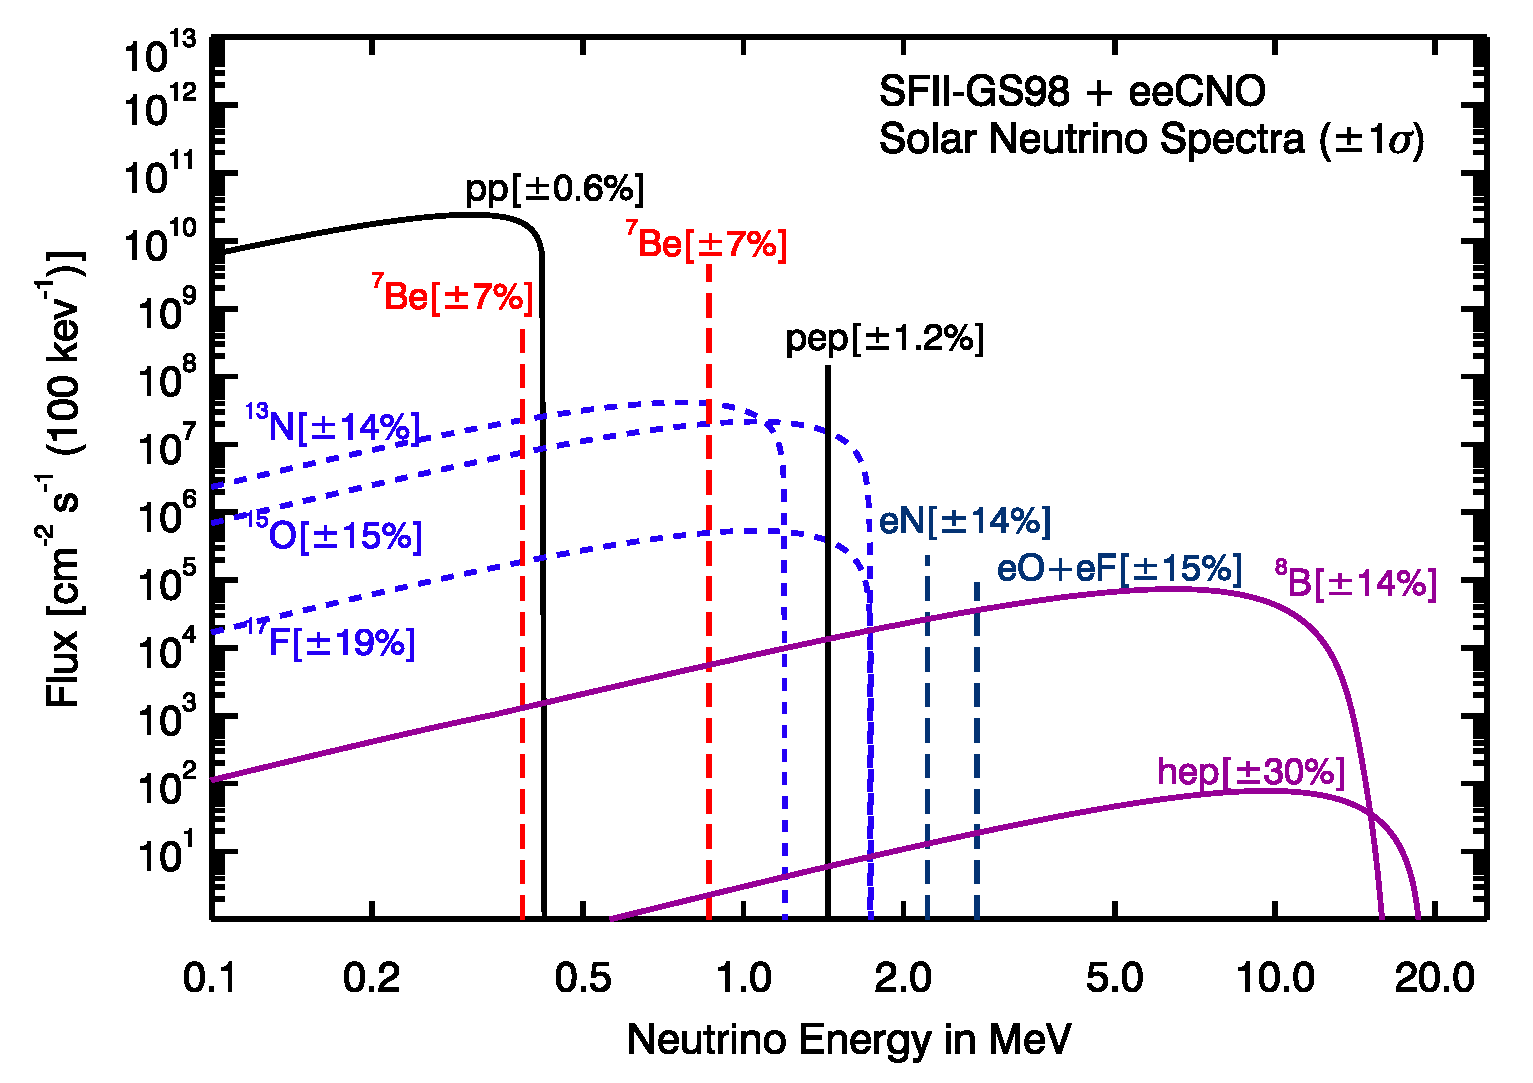
\includegraphics[width=0.85\linewidth]{thesis/6_figures/theory/figure3}
    \caption[The solar neutrino flux produced by all the reactions inside Sun's core]{Solar neutrino flux produced by all the reactions inside the Sun's core. Taken from \cite{serenelliAliveWellShort2016}.}
    \label{fig:sun_flux}
\end{figure}

Neutrinos from the Sun come from multiple reactions inside the Sun's core. An energy spectrum of the neutrino flux is presented in \autoref{fig:sun_flux}. The detector used the capture process $\PGne + ^{37}\mathrm{Cl} \to ^{37}\mathrm{Ar} + \Pem$, with a threshold of \SI{814}{keV}, making only $^7$Be and $^8$B flux detectable by the experiment. The produced $^{37}$Ar decayed in $\sim\SI{34.8}{days}$ and was counted by means of a proportional chamber. Despite the huge number of neutrinos from solar flux $\sim\SI{6e10}{cm^{-2}\ s^{-1}}$, only 1.7 events were expected each day \cite{bahcallStandardSolarModels1982,bahcallNewSolarOpacities2005}; however, the total flux collected by the Homestake Mine experiment amounted to an observed flux of \num{0.48(4)} neutrino interactions per day \cite{clevelandMeasurementSolarElectron1998}. This anomalous measurement is referred to the ``solar neutrino problem''. To investigate the origin of the ``solar neutrino problem'' other components of the $\Pp\Pp$ and CNO processes in the Sun's core,  other experiments were developed, with the aim of investigating the lower part of the energy spectrum. In particular, neutrinos from the $\Pp\Pp$ chain are the most abundant, so they were targeted to clarify this problem. In order to measure these neutrinos, the threshold had to be lowered. Using gallium, or gallium-doped targets, the neutrino capture process $\PGne + ^{71}\mathrm{Ga} \to ^{71}\mathrm{Ge} + \Pem$, with a threshold energy of \SI{233}{keV} it is possible to detect neutrinos from the $\Pp\Pp$ chain. Three experiments followed this idea: the SAGE experiment at Baksan \cite{collaborationMeasurementSolarNeutrino1999}, using \SI{50}{t} of liquid metallic gallium, and the GALLEX \cite{hampelGALLEXSolarNeutrino1999} experiment at \emph{Laboratori Nazionali del Gran Sasso} (LNGS), using gallium chloride, $\mathrm{GaCl_3}$. The GALLEX experiment was followed by the GNO experiments, and their data was used for a combined analysis \cite{hampelGALLEXSolarNeutrino1999,altmannGNOSolarNeutrino2000}. These results highlighted that also for this lower region of the energy flux, the model was inconsistent with the data.  The same was shown by the results from the SAGE collaboration \cite{collaborationMeasurementSolarNeutrino1999}.

The landscape evolved in 1998 with the observation of atmospheric neutrinos by the Kamiokande and Super-Kamiokande detectors. Where the radiochemical detectors measure the reaction rate integrated between extractions, the real-time measurement of solar neutrinos was possible with this experiment. The Kamiokande detector was a \SI{3000}{t} water-Cherenkov detector in the Kamioka mine. Super-Kamiokande (SK, for short), the successor of Kamiokande, started operation in 1996. It is a large upright cylindrical water Cherenkov detector containing \SI{50}{kt} of pure water. An inner volume of \SI{32}{kt} of water was surrounded by \num{11000} photomultiplier tubes (PMT), detecting the Cherenkov radiation from the particles inside the volume. Both Kamiokande and Super-Kamiokande can detect solar neutrinos using neutrino-electron elastic scattering (ES), $\PGn_\ell\Pem \to \PGn_\ell\Pem$. The results of Kamiokande and SK for $\PGne$ES events still showed a decrease of the observed flux $(\mathrm{2.308\pm0.020(stat.)^{+0.039}_{-0.040}(syst.)})\times \num{e6}$ \si{cm^{-2}\ s^{-1}} \cite{super-kamiokandecollaborationSolarNeutrinoMeasurements2016}, with respect to the expected flux of \SI{5.46+-0.66}{cm^{-2}\ s^{-1}}. %This constitutes the ``atmospheric neutrino problem''. 

% atmospheric neutrino anomaly...
The Kamioka water Cherenkov detector, as well as the Irvine-Michigan-Brookhaven (IMB) water Cherenkov detector, were also able to detect, other than electrons and electron neutrinos coming from the Sun's core, muons, and muon neutrinos. Those are predicted to be originating in Earth's atmosphere. Those experiments observed a deficit \cite{hirataExperimentalStudyAtmospheric1988, casperMeasurementAtmosphericNeutrino1991} of neutrinos from what was expected. This constitutes the ``atmospheric neutrino problem''. Atmospheric neutrinos come from interactions between cosmic rays and nuclei in the atmosphere, leading to the production of charged mesons, which then decay. One of the leading channels of this chain is the pion decay, $\PGppm\to\PGmpm+\brabar{\PGnGm}$, and the subsequent muon decay, $\PGmpm \to \Pepm + \brabar{\PGnGm} + \brabar{\PGne}$, implying  a flavour ratio $(\PGne + \PAGne) / (\PGnGm + \PAGnGm) = 1/2$. 

The solution for this ``atmospheric neutrino problem'' came directly with the SK detector, by following the hypothesis that neutrinos do oscillate, and hence that a deficit of muon neutrinos had to be found as an increase in the population of electron and tau neutrinos. The data collected by SK showed a good agreement for atmospheric neutrinos assuming a two-flavour oscillation \cite{ashieEvidenceOscillatorySignature2004}, with $\sin[2](2\theta) > 0.90$ and $\SI{1.9e-3}{eV^2} < \Delta m^2 < \SI{3e-3}{eV^2}$ at \SI{90}{\percent} confidence level. The confirmation for this will come from subsequent experimental efforts, especially from the OPERA detector working at the Laboratori Nazionali del Gran Sasso (LNGS), detecting neutrinos from the CERN Neutrinos to Gran Sasso (CNGS) beam --- it did, in fact, detect tau neutrinos \cite{collaborationDiscoveryTauNeutrino2015} from the CNGS $\PGnGm$-disappearance. 

The solution for the ``solar neutrino problem'' came in the early 2000s, with the experimental results by the Sudbury Neutrino Observatory (SNO, for short) \cite{collaborationMeasurementRateNu_e2001}. This experiment used \SI{1000}{t} of heavy water, $\mathrm{D_2O}$, contained in a spherical vessel surrounded by a $\mathrm{H_2O}$ shield. An array of PMTs looked at the Cherenkov radiation produced in both $\mathrm{D_2O}$ and $\mathrm{H_2O}$. This way the detector was able to look for multiple signatures of $^8$B from the Sun's core: in addition to ES scattering in water, heavy water allowed for the detection of CC $\PGne + \HepParticle{d}{}{} \to \Pem + \Pp+\Pp$, and NC $\PGn_\ell + \HepParticle{d}{}{} \to \PGn_\ell + \Pn+\Pp$, where $\ell = \Pe, \PGm, \PGt$ are all the SM neutrino flavours. Therefore, by comparing the three fluxes (ES, CC and NC), each sensible to one or more neutrino flavours, this detector was able to measure the full neutrino solar flux. The results of the SNO collaboration of CC and NC interactions, combined with the ES events collected by SK, published between 2001 and 2002, allowed the computation of the full flux of neutrinos from the Sun, highlighting that flavour conversion happened also in neutrinos \cite{collaborationDirectEvidenceNeutrino2002, collaborationMeasurementRateNu_e2001, collaborationSolar8BHep2001}. The final test came with the knowledge of neutrino oscillation in matter, through the MSW effect. The mass splitting reported by the SAGE \cite{abdurashitovMeasurementSolarNeutrino2009} and GALLEX+GNO \cite{altmannCompleteResultsFive2005} experiments was in the order of $\Delta m^2 \sim \SI{e-5}{eV^2}$, with the oscillation amplitude $\sin[2](2\theta)\sim0.3$. 

\begin{figure}
    \centering
    \includegraphics[width=0.85\linewidth]{thesis/6_figures/theory/pnt_SNO+SK}
    \caption[SNO+SK results for the ``solar neutrino problem'']{Fluxes of $^8$B solar neutrinos, $\phi(\PGne)$, and $\phi(\HepParticle{\PGn}{\PGm,\PGt}{})$, deduced from the SNO’s CC, ES, and NC results. The standard solar model prediction \cite{bahcallStandardSolarModels1982,bahcallNewSolarOpacities2005} is also shown. The bands represent the $1\sigma$ error. The contours show the \SI{68}{\percent}, \SI{95}{\percent}, and \SI{99}{\percent} joint probability for $\phi(\PGne)$ and $\phi(\HepParticle{\PGn}{\PGm,\PGt}{})$. The figure is from \cite{snocollaborationElectronEnergySpectra2005}.}
    \label{fig:sno_results}
\end{figure}


%. Theory, to formalize all
\subsubsection{Flavour oscillation formalism}

In the standard model of particle physics, the flavour oscillation is closely related with the mass mechanism, i.e. how elementary particle get teir masses. This is the case for the hadronic sector, where the mass mechanism is linked with flavour oscillation via the $V_\mathrm{CKM}$ matrix \cite{peskinIntroductionQuantumField1995}.

In the case of neutrinos, there is not \emph{one} mechanism for their masses --- there are upper limits to their mass value \cite{navasReviewParticlePhysics2024}, but since no direct measurement has been made to date, no hypothesis is stronger than others. Any model that aims at providing a valid mechanism for neutrino masses, however, is successful in describing the oscillatory behaviour.  The key for describing why neutrinos oscillate lies in what is that we actually call ``neutrinos.'' We \emph{cannot} see neutrinos directly as we can, for example, in the case of muons or electrons: we have to look at the products of neutrino interactions to be able to say whether it was an electron neutrino, a muon neutrino or a tau neutrino. We usually call $\PGne, \PGnGm, \PGnGt$ neutrinos, but in order to be more formal, we should say that this is the flavour eigenstate basis. As for the quarks, the mass basis can be different from the flavour basis. We define the mass basis as $\PGn_1, \PGn_2, \PGn_3$. What I have just said, about neutrinos being only detectable through their interaction products, can be more formally expressed as follows. The flavour eigenstate basis of neutrinos is that which undergoes weak interaction; on the other hand, the mass eigenstate basis is that which undergoes time transformation, and the masses are their eigenvalues, dictating how an eigenstate evolves through time. We can express each base as a rotation of the other, using the complex-valuex Pontecorvo-Maki-Nakagawa-Sakata (PMNS) matrix, 
\begin{equation}
    \ket{\PGn_\alpha} = \sum_{i=1}^3 U_{\mathrm{PMNS},\ \alpha i}^* \ket{\PGn_i},\quad \ket{\PGn_i} = \sum_{\alpha=1}^3 U_{\mathrm{PMNS},\ \alpha i} \ket{\PGn_\alpha}, \label{eq:basis_rotation}
\end{equation} where the Greek indices indicate the flavour eigenstate basis, and the Roman ones indicate the mass eigenstate basis.

The complex-valued $U_\mathrm{PMNS}$ matrix can be expressed as the product of three rotations and a complex phase \begin{equation}
    \begin{aligned}
        U_\mathrm{PMNS} &= \begin{pmatrix}
            1 & 0 & 0\\
            0 & \cos\theta_{23} & \sin\theta_{23} \\
            0 & -\sin\theta_{23} & \cos\theta_{23} \\
        \end{pmatrix} \times \begin{pmatrix}
            \cos\theta_{13} & 0 & \sin\theta_{13}\ e^{-i\delta} \\
            0 & 1 & 0\\
            -\sin\theta_{23}\ e^{i\delta} & 0 & \cos\theta_{23} \\
        \end{pmatrix} \times\\ 
        &\hspace{7cm}\times \begin{pmatrix}
            \cos\theta_{12} & \sin\theta_{12} & 0\\
            -\sin\theta_{12} & \cos\theta_{12} & 0\\
            0 & 0 & 1\\
        \end{pmatrix}
    \end{aligned} \label{eq:PMNS}
\end{equation} where $\theta_{ij}$ are the rotation angles, and $\delta$ is the Charge-Partiy (CP) violating phase, often referred to as $\delta_\mathrm{CP}$. The theory, in the case neutrinos were Majorana particles\footnote{This is a delicate question; here I am making the hypothesis that three right-handed Majorana neutrinos exists. A model where more than $n=3$ Majorana neutrinos exists would require more parameters, thus the PMNS matrix would be different.}, would require two additional phases, $\alpha_1$ and $\alpha_2$. This is obtained by multiplying the PMNS matrix by \[\mathrm{diag}\qty(e^{i\alpha_1/2}, e^{i\alpha_2/2}, 1).\]

Given the rotations in \eqref{eq:basis_rotation}, neutrino oscillation arise from the time evolution of the massive eigenstates $\PGn_i$, in vacuum \cite{zuberNeutrinoPhysics2020} \begin{equation}
    \ket{\PGn_i, t} = e^{-i p \cdot x} \ket{\PGn_i, t_0 = 0} = e^{-i E\ t  + \vb p \cdot \vb x} \ket{\PGn_i, t_0 = 0}.\label{eq:time_evolution}
\end{equation}
Combining \eqref{eq:basis_rotation} and \eqref{eq:time_evolution} leads to the flavour basis to oscillate as the mass eigenstates evolve in time (hereafter, $\ket{\PGn_i} = \ket{\PGn_i, t = 0}$ and the same for the Greek indices), \begin{equation}
    \ket{\PGn_\alpha, t} = \sum_{i} U_{\alpha i}^* e^{-i E\ t  + \vb p \cdot \vb x} \ket{\PGn_i} = \sum_\beta \qty(\sum_{i} U_{\alpha i}^* e^{-i E\ t  + \vb p \cdot \vb x} U_{\beta i}) \ket{\PGn_\beta}. 
\end{equation} The probability of evolving from the initial state $\beta$ to the final state $\alpha$ at a given time $t$ is given by \begin{equation}
    \begin{aligned}
        P(\PGn_\alpha \to \PGn_\beta) &= \qty|\braket{\PGn_\beta}{\PGn_\alpha, t}|^2 = \qty|\sum_i\sum_j U^*_{\alpha i}U_{\beta j} \braket{\PGn_j}{\PGn_i, t}|^2 = \\
        & = \delta_{\alpha\beta} - 4\sum_{i<j} \Re[U_{\alpha i} U_{\beta i}^* U_{\alpha j}^* U_{\beta j}] \sin[2](1.26 \ \frac{\Delta m^2_{ij} }{\si{eV^2}}\ \frac{L/E}{\si{m/MeV}}) + \\
        &\qquad\qquad + 2 \sum_{i<j} \Im[U_{\alpha i} U_{\beta i}^* U_{\alpha j}^* U_{\beta j}] \sin(2\times1.26 \ \frac{\Delta m^2_{ij} }{\si{eV^2}}\ \frac{L/E}{\si{m/MeV}}). \label{eq:oscillation_nbody}
    \end{aligned}
\end{equation} We have made the assumptions that, for $m_i \ll p_i$, since $E = \sqrt{p^2 + m^2}$, $\qty|\vb p|$ tends to $E$, and also \[
    E = \sqrt{p^2 + m^2} \simeq p + \frac{m^2}{2p} \simeq p + \frac{m^2}{2E}.
\] It is important to highlight --- especially for reasons I will present later on (see \autoref{sec:anomalies}) --- that no hypothesis about the number of neutrinos has been made to obtain such oscillation probability. Thus, equation \eqref{eq:oscillation_nbody} is valid for any number $N$ of neutrinos family, as long as the mixing PMNS matrix is $N\times N$. 

Looking closely at the contributions of \eqref{eq:oscillation_nbody}, we highlight three components. The first $\delta_{\alpha\beta}$ is equivalent to not having any oscillation --- becomes important in disappearance studies. The second term, proportional to $\Re[U_{\alpha i} U_{\beta i}^* U_{\alpha j}^* U_{\beta j}]$ is closely related to the mixing angles, but is not sensible in any way to the $\delta_\mathrm{CP}$ CP violating complex phase. This is instead related --- thereby measured by looking at --- the $\Im[U_{\alpha i} U_{\beta i}^* U_{\alpha j}^* U_{\beta j}]$ term of the equation. 

Finally, some remarks are necessary about the equation in \eqref{eq:oscillation_nbody}. The first remark is regarding the Majorana phases, intrduced briefly after \eqref{eq:PMNS}. As it is clear if we further develop the related math of eq. \eqref{eq:oscillation_nbody}, the $N$-flavour oscillation is not sensitive to the Majorana phases, for which a different type of research is required: this is still strictly related to the problem of neutrino masses and also to the CP violation problem \cite{brancoMajoranaNeutrinosCP1986, navasReviewParticlePhysics2024}, but not dealt with in this thesis.

A second remark is that, as already pointed out when discussing the solution of the ``solar neutrino problem'' before, the computation presented in  \eqref{eq:oscillation_nbody} is valid only for neutrinos propagating through vacuum space. In the case of propagation through matter, it is important to consider the effect such interaction might produce and its impact on neutrino oscillation. This effect was first computed by Mikheyev-Smirnov-Wolfenstein, hence the name MSW effect. This effect shows, starting from the hypothesis that neutrinos in matter interact coherently, how the difference between the electron neutrino flavour --- which can interact both through CC and NC coherent scatter with the nuclei ---, and the muon/tau neutrino flavours --- interacting only through NC coherent scattering --- result in a difference of their oscillation probability \cite{mikheevResonantAmplificationNeutrino1986, mikheyevResonanceAmplificationOscillations1985, wolfensteinNeutrinoOscillationsMatter1978}. This effect, while not essential for short baseline experiments such as the SBN program, is core for long baseline experiments, like the Deep Underground Neutrino Experiment \cite{kellyMatterDensityProfile2018}, and for solar neutrino experiments, which have to take into account the oscillation probability induced by neutrinos crossing the Sun's radius. 

The final remark is about the experimental values of the mass splitting. As I will show later on, with the current status of neutrino oscillation experiments, we have identified two values of mass splitting: one coming from the best fit of atmospheric neutrino oscillations ($\PGnGm\leftrightarrow\PGnGt$ oscillations), which I will call $\qty|\Delta m^2_\mathrm{Atmospheric}|$, and the other from the best fit of solar neutrino oscillations (mainly $\PGne\leftrightarrow\PGnGm$ oscillations), which I will call $\Delta m^2_\mathrm{Solar}$. The peculiarity is that these values show two orders of magnitude of difference, \begin{equation}
    \qty|\Delta m^2_\mathrm{Atmospheric}| \simeq \SI{e-3}{eV^2} \gg \Delta m^2_\mathrm{Solar} \simeq \SI{e-5}{eV^2}.
\end{equation} Since we cannot know, for the atmospheric oscillations, the sign of the mass splitting, there are two possible pictures. The first, called normal ordering or normal hierarchy (NO/NH), assumes a positive sign for both, and so $m_1^2 \leq m_2^2 \leq m_3^2$. The other option assumes a negative sign for the atmospheric mass splitting, and thus $m_3^2 \leq m_1^2 \leq m_2^2$. \autoref{fig:ordering} shows an illustration of both NO (left) and IO (right). The mass splitting difference also allows, in most cases, to distinctly separate the two oscillation frequencies. This is why, for most short- and long-baseline experiments, it is usually more convenient to approximate the oscillation as a two-flavour oscillation. 

\begin{figure}
    \centering
    \begin{tikzpicture}[
        nue/.style={fill=Red!70!white},
        numu/.style={fill=ForestGreen!65!white},
        nutau/.style={fill=MidnightBlue!65!white},
        scale=0.75
    ]

        %%%%%%%%%%%%%%%%%%%%%%%%%%%%%%%%%%%%%%%%%%%%%%%%%%%%%%%%%%%%%%%%%%%%%%%%%%%%%%%%
        %%%%%% NORMAL MASS ORDERING %%%%%%%%%%%%%%%%%%%%%%%%%%%%%%%%%%%%%%%%%%%%%%%%%%%%
        %%%%%%%%%%%%%%%%%%%%%%%%%%%%%%%%%%%%%%%%%%%%%%%%%%%%%%%%%%%%%%%%%%%%%%%%%%%%%%%%

        \node[text centered] at (-3,0) {Normal ordering};
        \node[text centered] at (-0.5,0) {$\delta_\mathrm{CP}$};

        \node[text centered] at (-5.5, -.75)  {$\PGn_3$};
        \node[text centered] at (-5.5, -3.75) {$\PGn_2$};
        \node[text centered] at (-5.5, -4.75) {$\PGn_1$};

        \fill[nue] (-5,-.5) -- (-4.75,-.5) -- (-4.75,-1) -- (-5,-1) -- cycle;
        \fill[numu] (-4.75,-.5) -- (-3.,-.5) -- (-3.,-1) -- (-4.75,-1) -- cycle;
        \fill[nutau] (-3.,-.5) -- (-1,-.5) -- (-1,-1) -- (-3.,-1) -- cycle;

        \draw[black] (-5,-.5) rectangle (-1,-1);

        \node[text centered] at (-.65, -.5) {\small$\pi$};
        \node[text centered] at (-.65, -1) {\small 0};

        \fill[nue] (-5,-3.5) -- (-4.,-3.5) -- (-4.,-4) -- (-5,-4) -- cycle;
        \fill[numu] (-4.,-3.5) -- (-2.15,-3.5) -- (-3,-4) -- (-4,-4) -- cycle;
        \fill[nutau] (-2.15,-3.5) -- (-1,-3.5) -- (-1,-4) -- (-3.,-4) -- cycle;

        \draw[black] (-5,-3.5) rectangle (-1,-4);

        \node[text centered] at (-.65, -3.5) {\small$\pi$};
        \node[text centered] at (-.65, -4) {\small 0};

        \fill[nue] (-5,-4.5) -- (-2.575,-4.5) -- (-2.575,-5) -- (-5,-5) -- cycle;
        \fill[numu] (-2.575,-4.5) -- (-2.2,-4.5) -- (-1.25,-5) -- (-2.575,-5) -- cycle;
        \fill[nutau] (-2.2,-4.5) -- (-1,-4.5) -- (-1,-5) -- (-1.25,-5) -- cycle;

        \draw[black] (-5,-4.5) rectangle (-1,-5);

        \node[text centered] at (-.65, -4.5) {\small$\pi$};
        \node[text centered] at (-.65, -5) {\small 0};

        \draw[gray, line width=1mm] (-6.25, -4.85) -- (-6.25, -3.65);
        \draw[gray, line width=1mm] (-6, -.65) -- (-6, -3.85);

        \node[] at (-7.65, -4.25) {
            \begin{minipage}{1.75cm}
                \raggedleft
                Solar\\
                $\sim \SI{e-5}{eV^2}$
            \end{minipage}
        };

        \node[] at (-4.25, -2.25) {
            \begin{minipage}{1.85cm}
                Atmospheric\\
                $\sim \SI{e-3}{eV^2}$
            \end{minipage}
        };

        %%%%%%%%%%%%%%%%%%%%%%%%%%%%%%%%%%%%%%%%%%%%%%%%%%%%%%%%%%%%%%%%%%%%%%%%%%%%%%%%
        %%%%%% INVERTED MASS ORDERING %%%%%%%%%%%%%%%%%%%%%%%%%%%%%%%%%%%%%%%%%%%%%%%%%%
        %%%%%%%%%%%%%%%%%%%%%%%%%%%%%%%%%%%%%%%%%%%%%%%%%%%%%%%%%%%%%%%%%%%%%%%%%%%%%%%%

        \node[text centered] at (+3,0) {Inverted ordering};
        \node[text centered] at (+5.5,0) {$\delta_\mathrm{CP}$};

        \node[text centered] at (0.5, -.75)  {$\PGn_2$};
        \node[text centered] at (0.5, -1.75) {$\PGn_1$};
        \node[text centered] at (0.5, -4.75) {$\PGn_3$};

        \fill[nue] (1,-.5) -- (2.,-.5) -- (2.,-1) -- (1,-1) -- cycle;
        \fill[numu] (2.,-.5) -- (3.85,-.5) -- (3,-1) -- (2,-1) -- cycle;
        \fill[nutau] (3.85,-.5) -- (5,-.5) -- (5,-1) -- (3.,-1) -- cycle;

        \draw[black] (1,-.5) rectangle (5,-1);

        \node[text centered] at (5.35, -.5) {\small$\pi$};
        \node[text centered] at (5.35, -1) {\small 0};

        \fill[nue] (1,-1.5) -- (3.425,-1.5) -- (3.425,-2) -- (1,-2) -- cycle;
        \fill[numu] (3.425,-1.5) -- (3.8,-1.5) -- (4.75,-2) -- (3.425,-2) -- cycle;
        \fill[nutau] (3.8,-1.5) -- (5,-1.5) -- (5,-2) -- (4.75,-2) -- cycle;

        \draw[black] (1,-1.5) rectangle (5,-2);

        \node[text centered] at (5.35, -1.5) {\small$\pi$};
        \node[text centered] at (5.35, -2) {\small 0};

        \fill[nue] (1,-4.5) -- (1.25,-4.5) -- (1.25,-5) -- (1,-5) -- cycle;
        \fill[numu] (1.25,-4.5) -- (3.,-4.5) -- (3.,-5) -- (1.25,-5) -- cycle;
        \fill[nutau] (3,-4.5) -- (5,-4.5) -- (5,-5) -- (3.,-5) -- cycle;

        \draw[black] (1,-4.5) rectangle (5,-5);

        \node[text centered] at (5.35, -4.5) {\small$\pi$};
        \node[text centered] at (5.35, -5) {\small 0};

        \draw[-*, Red!65!black, shorten >=-2pt] (-4, -5.5) node[below, text centered] {$\PGne$} -- (-4, -5);
        \draw[-*, ForestGreen!65!black, shorten >=-2pt] (-2, -5.5) node[below, text centered] {$\PGnGm$} -- (-2, -5);
        \draw[-*, MidnightBlue!65!black, shorten >=-2pt] (-1.15, -5.5) node[below, text centered] {$\PGnGt$} -- (-1.15, -5);

        \draw[gray, line width=1mm] (6.1, -4.85) -- (6.1, -1.65);
        \draw[gray, line width=1mm] (5.85, -.65) -- (5.85, -1.85);

        \node[] at (7.25, -.85) {
            \begin{minipage}{1.75cm}
                Solar\\
                $\sim \SI{e-5}{eV^2}$
            \end{minipage}
        };

        \node[] at (4.25, -3.25) {
            \begin{minipage}{2cm}
                \raggedleft
                Atmospheric\\
                $\sim \SI{e-3}{eV^2}$
            \end{minipage}
        };

        \draw[-Latex, very thick] (-7.25, -2.) node[below] {$m_\PGn^2$} -- (-7.25, -0.5);
        
    \end{tikzpicture}
    \caption[Neutrino mass ordering]{The two cases for neutrino mass ordering:  the normal ordering, on the left, and the inverted ordering, on the right. The shaded area represents the mixing angles, or the fraction of each flavour in the masses eigenstates. Additionally, the dependence on the CP violating phase effect is shown, with its value ranging from 0 to $\pi$. Adapted from \cite{menaUnifiedGraphicalSummary2004}.}
    \label{fig:ordering}
\end{figure}

%. Presenta status
\subsubsection{Present status}

To quantify neutrino oscillations is to measure the parameters of the PMNS matrix. As we can read from \eqref{eq:PMNS}, it depends on three angles and a complex phase, so in order to measure it correctly, multiple experimental measurements must be carried out. Additionally, one aims at knowing the precise value of the mass splittings. Each parameter can be accessed by exploiting different neutrino sources in order to vary the baseline and the energy or the $L/E$ ratio of the measured interaction to pinpoint each parameter in the phase space. Additionally, oscillation measurements are classified either as ``appearance'' experiments, where the oscillation from one flavour $\alpha$ to another flvour $\beta$ is measured, or as ``disappearance'' measurements, where the probability $P(\PGn_\alpha \to \PGn_\alpha) = 1 - \sum_{\beta\neq\alpha} P(\PGn_\alpha \to \PGn_\beta)$ of getting the same flavour at different distances from the sources is tested. 

The distance of the detector from the experimental source is usually selected to maximise the sensitivity to a precise mass splitting, $\Delta m^2 \sim E/L$. 

Recently, the precision with which these parameters are determined reached a percent value, allowing neutrino oscillation physics to move from ``discovery'' field to the ``precision'' era. 

\paragraph{Solar neutrino observations} Solar neutrinos have been the first probe for neutrino oscillations and still are an interesting source to both study neutrino oscillations and also to test neutrino interaction in matter. The $E/L$ of neutrinos from the sun, given that $\SI{233}{keV} \leq E_\PGn \lesssim \si{MeV}$, limits the values of mass splitting to those of the solar mass splitting, $\Delta m^2_\mathrm{Solar} \sim \SI{e-5}{eV^2}$. This limits oscillation to mainly a two-flavour oscillation $\PGne\leftrightarrow\PGnGm$, so that mainly $\sin\theta_{12}$ is accessible. The complete picture is obtained from multiple years of observations from multiple detectors, leading to a best value of $\Delta m_{21}^2 \simeq \qtyrange{6.92e-5}{8.05e-5}{eV^2}$ and $\sin^2\theta_{12} \simeq \numrange{0.275}{0.345}$ at $3\sigma$. These results come from combining the results from the Soviet-American Gallium Experiment (SAGE) \cite{abdurashitovMeasurementSolarNeutrino2009}, the gallium experiment (GALLEX), combined with the Gallium Neutrino Observatory (GNO) \cite{altmannCompleteResultsFive2005}, the Kamiokande and SK experiments \cite{collaborationSolarNeutrinoMeasurements2024}, joined by the BOREXINO experiment \cite{agostiniExperimentalEvidenceNeutrinos2020} and the KamLAND experiment \cite{kamlandcollaboration$^7mathrmBe$SolarNeutrino2015}. 

\paragraph{Atmospheric neutrinos} The $L/E$ ratio for neutrinos generated by pion decay in the atmosphere allows exploring the $\PGnGm\leftrightarrow\PGnGt$ oscillation phase space that is characterised by a mass splitting $|\Delta m_{32}^2| = |\Delta m_\mathrm{Atmospheric}^2| \sim \SI{e-3}{eV^2}$, and so allows for the determination of $\sin\theta_{23}$. Atmospheric neutrino oscillations have been studied by the Kamiokande experiment \cite{hirataExperimentalStudyAtmospheric1988} and its successor, Super-Kamiokande \cite{ashieEvidenceOscillatorySignature2004}, by the MACRO experiment \cite{collaborationMatterEffectsUpwardGoing2001}, and also by neutrino telescopes, such as the ANTARES experiment and the IceCube experiment. Novel experiments will join this research, such as the KM3NeT-ORCA telescope, the successor of the ANTARES experiment, the Hyper-Kamiokande experiment, the JUNO experiment, and the DUNE experiment. 

\paragraph{Accelerator neutrinos} A similar phase space to that of atmospheric neutrino oscillations can be explored by the accelerator neutrino experiments, especially at long baselines. Accelerator neutrinos can be interesting still, since they provide a large flux with a great purity of the beam. Conventional neutrino beams from accelerators are produced by colliding high-energy particles onto a target --- usually $\Pp$ on a $^7$Be target --- producing $\PGp$ and $\PK$, which then decay into neutrinos. The branching ratio of $\PGpp \to \PGmp\PGnGm$ is $\sim\SI{100}{\percent}$, with minimal contamination from $\PGne$ and $\PAGne$, coming from kaon decays. The values of neutrino energy and baselines are chosen to maximise the oscillation probability, either for studying the atmospheric mass splitting $\qty|\Delta m_{21}^2| \simeq \SI{2.5e-3}{eV^2}$, with the first oscillation maximum at $L/E \simeq \SI{500}{GeV/km}$, or for testing the $\Delta m^2 \sim \SI{1}{eV^2}$ splitting at $\sim \SI{1}{km}$ baselines. 

The present landscape of the accelerator neutrino experiments is vast, from the first experiments being the K2K and MINOS experiments --- exploring the values of $\Delta m_{31}^2$ and $\Delta m_{32}^2$, studying the $\PGnGm$-disappearance channel --- to their successor, the T2K experiment, successor of the K2K experiment, employing Super-Kamiokande as its far detector at \SI{295}{km}, and the NOvA experiment, collecting neutrinos from the Neutrino at the Main Injector (NuMI) beam at a baseline of \SI{810}{km}. Both T2K and NOvA measured $\Delta m_{31}^2$, $\Delta m_{32}^2$ , and $\sin\theta_{23}$ by measuring oth the $\PGne$-appearance and $\PGnGm$-disappearance channels from a pure $\PGnGm$ beam \cite{abeObservationElectronNeutrino2014, collaborationMeasurementsNeutrinoOscillation2023, collaborationConstraintsOscillationParameters2017}. Additionally, both experiments were capable of measuring the $\delta_\mathrm{CP}$ violating phase of the PMNS matrix. The T2K collaboration showed a preference towards $\delta_\mathrm{CP}\sim\pi/2$ \cite{collaborationMeasurementsNeutrinoOscillation2023}, whereas the NOvA collaboration showed a preference towards $\delta_\mathrm{CP}\sim3\pi/2$ \cite{collaborationConstraintsOscillationParameters2017}. 

\paragraph{Reactor antineutrinos} Nuclear fission reactors give a substantial flux of electron antineutrinos in the \si{MeV} region, through $\beta$-decay of radioactive isotopes created during the fission process, primarily $^{235}$U, $^{238}$U, $^{239}$Pu, and $^{241}$Pu; $\PAGne$ are then detected at different baselines$\sim\SI{1}{km}$. Charged current events cannot happen, given the neutrino energies, for $\PAGnGt$ or $\PAGnGt$ since they require more energy to produce $\PGm$ or $\PGt$ in the final state than what is accessible, so flavour oscillation for such experiments is only accessible through the $\PAGne$-disappearance channel. The detection mechanism is from the inverse beta decay $\Pp + \PAGne \to \Pep + \Pn$, where the signal from the prompt $\Pep$ and the $\PGg$ (with the energy depending on the type of scintillator; \SI{2.2}{MeV} for hydrogen, \SI{8}{MeV} when it is loaded with gallium) from the thermalisation of the neutron helps separate it from the background. 

The Kamioka Liquid Scintillator Antineutrino Detector (KamLAND) experiment was one of the first milestones in neutrino physics, detecting neutrinos from multiple nuclear reactors at $\sim \SI{180}{km}$ from the detector, and detected a ratio of observed inverse $\beta$ decay over the predicted flux of $\mathrm{0.611 \pm 0.085(stat) \pm 0.041(syst)}$ \cite{collaborationFirstResultsKamLAND2003}, showing evidence for $\PAGne$-disappearance at \SI{99.95}{\percent} confidence level. 

Reactor antineutrino experiments also showed very high sensitivity to the $\theta_{13}$ mixing angle. This is possible by looking at a short baseline $\sim \SI{1}{km}$: such searches have been performed by the Double Chooz experiment \cite{abeIndicationDisappearanceReactor2012}, the Daya Bay experiment \cite{anObservationElectronantineutrinoDisappearance2012}, and the RENO experiment \cite{kimObservationReactorElectron2012}, which found, respectively, \begin{align}
    &\begin{aligned}
        \sin^22\theta_{13} &= \mathrm{0.086 \pm 0.041 (stat) \pm 0.030 (syst)},\\
        & \text{or}\ 0.017 < \sin^22\theta_{13} < 0.16\ \text{at \SI{90}{\percent} CL}
    \end{aligned} && \text{(Double Chooz)}\\
    &\sin^22\theta_{13} = \mathrm{0.092 \pm 0.016(stat) \pm 0.005(syst)} && \text{(Daya Bay)}\\
    &\sin^22\theta_{13} = \mathrm{0.113 \pm 0.013(stat) \pm 0.019(syst)} && \text{(RENO)}
\end{align} 

\section{Short baseline anomalies}\label{sec:anomalies}

It is clear at this point that the picture of neutrino flavour oscillation is well established, from the empirical point of view, leading to the clear necessity of a ``minimal'' extension of the standard model in order to introduce neutrino masses. Since the nature of neutrinos is very different from other particles of the standard model, generating their masses would require a novel mechanism. Multiple beyond SM physics (BSM) models have been developed, many of which would require the addition of particle content to the SM; however strong the evidence for neutrino masses is, no direct measurement has been made to date, and no model is preferred over the others. 

In addition to this dilemma, in the past twenty years the picture has been complicated by some anomalous observations that could be hinting at the possibility of a fourth neutrino state. This was suggested by a series of ``short-baseline'' experiments --- for which $L/E \sim \SI{10}{m}/\si{MeV}$ \cite{aceroWhitePaperLight2024}. 

The Liquid Scintillator Neutrino Detector (LSND) at Los Alamos Laboratories detected $\PAGne$ from oscillated $\PAGnGm$ using a liquid scintillator and observed an excess of electron antineutrinos, with a tension of $3.8\sigma$ from the model \cite{aguilarEvidenceNeutrinoOscillations2001}. This result was tested by the MiniBooNE experiment with different neutrino sources and at a different baseline, which claimed a similar result with a significance of $4.8\sigma$ \cite{collaborationCombined$n_mtoN_e$2012}. Reactor antineutrino measurements, which played a significant role in establishing the three-flavour oscillation paradigm for neutrinos, also observed a decrease in flux of electron antineutrinos at baseline distances $<\SI{100}{m}$, with a ratio to the prediction $R=\num{0.976+-0.024}$ \cite{mentionReactorAntineutrinoAnomaly2011} --- this is the ``reactor antineutrino anomaly''. Of equal importance in the discovery of flavour oscillation are the solar neutrino experiments. GALLEX and SAGE \cite{collaborationMeasurementSolarNeutrino1999, hampelGALLEXSolarNeutrino1999} employed radiochemical techniques to detect solar neutrinos with gallium; calibration was performed using megacurie radioactive sources and returned anomalous fluxes in the $\PGne$-disappearance channel, with an observed-expected ratio $R=\num{0.86\pm0.05}$, showing a $2.2\sigma$ statistical significance: this, corroborated by the results of the BEST experiment --- which increased this significance to $\sim4\sigma$ \cite{elliottGalliumAnomaly2023} --- constitutes the ``Gallium anomaly'' (or GA). The combination of these anomalies at short baselines of $\sim\SI{1}{km}$ hints at the existence of a fourth neutrino flavour with a mass splitting $\Delta m^2 \sim \SI{1}{eV}$. This, combined with the fact that only three ``active'' (i.e. interacting) families of neutrinos are compatible with the experimental results so far \cite{decampPreciseDeterminationNumber1990}, lead to the ``sterile'' neutrino hypothesis: a neutrino that does not undergo weak interaction and is subject to gravitational force.

\paragraph{Pion decay-at-rest accelerator experiments} Pion decay-at-rest provide with a very pure muon antineutrino flux with a mean energy of $E_\PAGn\simeq \SI{30}{MeV}$. As such, a detector placed at a relatively short baseline $\sim\SI{30}{m}$ is sensitive to oscillation with a mass splitting $\sim\SI{1}{eV^2}$. Two major experiments employed this technology to produce neutrino beams, the LSND (Liquid Scintillator Neutrino Detector) and the KARMEN (KArlsruhe Rutherford Medium Energy Neutrino) experiments. Of the two, LSND had the highest sensitivity and observed the ``LNSD anomaly''. The KARMEN experiment saw no evidence of such an anomaly, and it is thus considered a ``null'' experiment for the sterile neutrino framework \cite{collaborationUpperLimitsNeutrino2002}. 

The LSND experiment consisted of a cylindrical tank of \SI{8.3}{m} of height and a diameter of \SI{5.7}{m}, placed horizontally, filled with \SI{167}{metric\ ton} of mineral oil. LNSD detected electron antineutrinos from a beam of muon antineutrinos, produced by pions decaying at rest (DAR). The pions were produced by protons with $E_\Pp\simeq \SI{798}{MeV}$ hitting a target and stopped in water. The signal selection proceeded by looking at both the scintillation light and the Cherenkov light cone produced by the positron (see figure \ref{fig:LSND_detector} for a schematic illustration) correlated with a \SI{2.2}{MeV} photon signal produced by neutron capture. Scintillation and Cherenkov light were collected by means of 1220 PMTs. The LNSD detector collected data showing an excess of events of $\mathrm{87.9 \pm 22.4\ (stat) \pm 6.0\ (sys)}$, compatible with the hypothesis of a two-flavour oscillation $\PAGnGm\to\PAGne$. The fit pointed toward an oscillation amplitude of $\sin^22\theta_{\PGm\Pe} \simeq \num{0.003}$ and a mass splitting of $\Delta m^2 \simeq \SI{1.2}{eV^2}$, resulting in the allowed regions at \SI{90}{\percent} CL and \SI{99}{\percent} CL shown in figure \ref{fig:LSND_lhd} \cite{lsndcollaborationEvidenceNeutrinoOscillations2001}. 

\begin{figure}
    \centering
    \subfloat[]{\includegraphics[width=0.5\linewidth, trim={0 -4cm 0 0}]{thesis/6_figures/anomalies/LNSD.pdf}\label{fig:LSND_detector}}
    \subfloat[]{\includegraphics[width=0.5\linewidth]{thesis/6_figures/anomalies/Fig27_lhd.pdf}\label{fig:LSND_lhd}}
    \caption[The LNSD detector and results]{\ref{sub@fig:LSND_detector} Illustration of the LNSD detector at the Los Alamos Laboratories. In the illustration an electron antineutrino interaction is displayed, with both the prompt scintillation light and Cherenkov cone from the positron, as well as the light emitted by the subsequent neutron capture. Adapted from \cite{louisThousandEyesStory1997}. \ref{sub@fig:LSND_lhd} Allowed regions from the LNSD fit of the sterile neutrino hypothesis in the $(\Delta m^2, \sin^22\theta)$ phase space of the oscillation with this state. Taken from \cite{lsndcollaborationEvidenceNeutrinoOscillations2001}}
    \label{fig:LSND}
\end{figure}

\paragraph{Pion decay-in-flight accelerator experiments} LNSD's evidence for this oscillation prompted subsequent searches that needed to be independent. This is why pion decay-in-flight (DIF) was selected as a valid production mechanism: it produces a pure $\brabar{\PGnGm}$ beam with higher energy, providing the opportunity for an independent test at a higher baseline. This was accomplished using the Booster Neutrino Beam (BNB) with the MiniBooNE Cherenkov detector at the Fermi National Accelerator Laboratories (Fermilab) in Illinois, providing a \SI{99.5}{\percent} pure muon neutrino beam with a mean energy of $\sim \SI{700}{MeV}$. The design of this experiment was made to allow the phase space to align with that of the LNSD experiment: $E/L \sim \SI{30}{MeV}/\SI{30}{m}$ for the LNSD experiment, so the same was accomplished by placing the MiniBooNE detector at \SI{540}{m}. The MiniBooNE detector consisted of a single tank containing \SI{818}{\tonne} of mineral oil. The detection was performed looking for Cherenkov radiation inside the tank with 1520 PMTs, and the Cherenkov signature was used to separate between $\PGne$CC and $\PGnGm$CC events; this selection suffered from backgrounds coming mainly from NC interactions inside the tank and NC $\PGpz$ interactions where one photon from the $\PGpz$ decay is not identified. The MiniBooNE experiment took data from 2002 to 2019, collecting a total of \SI{18.75e20}{POT} (protons-on-target) interactions with both a neutrino mode and an antineutrino mode, showing an excess of events in the signal region $\SI{200}{MeV} < E_\PGn^\mathrm{QE} < \SI{475}{MeV}$, with a statistical significance of $4.8\sigma$ \cite{collaborationUpdatedMiniBooNENeutrino2021}. This excess is known by the name of Low Energy Excess, LEE, shown in \autoref{fig:MiniBooNE}. 

\begin{figure}
    \centering
    \includegraphics[width=0.9\linewidth]{thesis/6_figures/anomalies/miniboone_results.pdf}
    \caption[MiniBooNE detector and results]{(left) Neutrino energy distribution of $\PGne$CC QE events recorded by the MiniBooNE detector in neutrino mode. The dashed line show the best fit in the sterile neutrino scenario. (right) An example of the type of interactions inside the detector, with different signatures for different final state interactions.}
    \label{fig:MiniBooNE}
\end{figure}

\paragraph{Reactor antineutrino experiments} In the most simple sterile neutrino picture (more about this later in \autoref{sec:sterile_theory}) where one sterile neutrino is assumed, non-zero $\PGne$ disappearance oscillation in neutrinos from reactors should be possible, with detectors placed $<\SI{100}{m}$ from the neutrino source. In such experiments at ILL-Grenoble, Goesgen, Rovno, Krasnoyarsk, Savannah River and Bugey \cite{mentionReactorAntineutrinoAnomaly2011}, the measured rate of $\PGne$ was found to be in reasonable agreement with that predicted from the reactor antineutrino spectra, though slightly lower than expected, with the measured/expected ratio at $R=\num{0.976+-.024}$, representing a $2.7\sigma$ deviation from the prediction. This is known as the ``reactor antineutrino anomaly'' (RAA). The additional measurements by the long-baseline detectors KamLAND and CHOOZ provided a stricter lower result of such ratio, at $R=\num{0.943 +- 0.023}$, deviating from the unity with a statistical significance of $\SI{98.6}{\percent}$ CL. 

\paragraph{Radioactive sources experiments} Radioactive sources are often used as calibration for different types of detectors. This was the case for both the GALLEX and SAGE solar neutrinos detectors. Such experiments employ natural radioactive sources, either $^{51}$Cr or $^{37}$Ar, which both produce electron neutrinos through electron capture processes \begin{align}
    \Pem + {}^{51}\mathrm{Cr} &\to {}^{51}\mathrm{V} + \PGne, && \text{(GALLEX)}\\
    \Pem + {}^{37}\mathrm{Ar} &\to {}^{37}\mathrm{Cl} + \PGne, && \text{(GALLEX, SAGE)}
\end{align} placed inside the detector, to calibrate the flux of electron neutrinos with respect to the rate of electron capture processes $\PGne + {}^{71}\mathrm{Ga} \to {}^{71}\mathrm{Ge} + \Pem$ observed. Both experiments observed a deficit of counts during the detector calibration with respect to the well-known and computed activities of the sources and the cross-section for the measurements, with average ratio $\overline R$ ranging from $\numrange{0.703 +- 0.078}{0.844 +- 0.031}$ \cite{giuntiGalliumAnomalyCritical2022}. A dedicated experiment was planned, Baksan Experiment on Sterile Transitions (BEST), where a larger deficit was observed, confirming the Gallium anomaly. The combined ratio show a statistical significance of $4\sigma$, with $\overline{R} = \num{0.80+-0.04}$. 

\subsection{The sterile neutrino hypothesis} \label{sec:sterile_theory}

The picture presented so far seems to hint, from multiple perspective, to the possibility of a sterile neutrino scenario. This requires the introduction of a fourth sterile --- i.e. not weakly interacting --- neutrino state, taking part in short baseline oscillation, with a mass splitting of $\Delta m^2 \sim \mathcal{O}(\SI{1}{eV^2})$. The need for this state to be ``sterile'' is required to minimally extend the SM, since the introduction of a massive weakly interacting particle with $m<m_\PZ/2$ would not be possible. 

I claimed before that the PMNS matrix size did not prevent neutrino oscillation from being possible in the current picture. Thus, the most general approach to introducing sterile particle content in the leptonic sector would be to add $N$ sterile neutrinos and consider a $(3+N)\times(3+N)$ PMNS matrix. This is correct and the most general way of introducing sterile neutrinos in the model, but to keep the number of parameters in the model as small as possible, it is effectively interesting to look at a ``simpler'' model, where only one additional sterile family is introduced. This $3+1$ paradigm, which is what I will consider moving forward, requires the introduction of a sterile state $\PGns$, and a basis of four massive neutrinos $\PGn_1, \dots, \PGn_4$, with the additional assumption that the fraction of $\PGns$ is extremely small for the first three mass eigenstates and near \SI{100}{\percent} for the fourth, as illustrated in \autoref{fig:ordering_NO_sterile}. 

\begin{figure}
    \centering
    \begin{tikzpicture}[
        nue/.style={fill=Red!70!white},
        numu/.style={fill=ForestGreen!65!white},
        nutau/.style={fill=MidnightBlue!65!white},
        nusterile/.style={fill=Gray!35!white},
        scale=0.75
    ]

        %%%%%%%%%%%%%%%%%%%%%%%%%%%%%%%%%%%%%%%%%%%%%%%%%%%%%%%%%%%%%%%%%%%%%%%%%%%%%%%%
        %%%%%% NORMAL MASS ORDERING %%%%%%%%%%%%%%%%%%%%%%%%%%%%%%%%%%%%%%%%%%%%%%%%%%%%
        %%%%%%%%%%%%%%%%%%%%%%%%%%%%%%%%%%%%%%%%%%%%%%%%%%%%%%%%%%%%%%%%%%%%%%%%%%%%%%%%

        \node[text centered] at (-3,4.5) {Normal ordering};
        \node[text centered] at (-0.25,4.5) {$\delta_\mathrm{CP}$};

        \node[text centered] at (-5.5, 3.75)  {$\PGn_4$};
        \node[text centered] at (-5.5, -.75)  {$\PGn_3$};
        \node[text centered] at (-5.5, -3.75) {$\PGn_2$};
        \node[text centered] at (-5.5, -4.75) {$\PGn_1$};

        \fill[nusterile] (-1,4) -- (-5,4) -- (-5,3.5) -- (-1,3.5) -- cycle;
        \fill[nue] (-.9,4) -- (-1,4) -- (-1,3.5) -- (-.9,3.5) -- cycle;
        \fill[numu] (-.825,4) -- (-.9,4) -- (-.9,3.5) -- (-.825,3.5) -- cycle;
        \fill[nutau] (-.75,4) -- (-.825,4) -- (-.825,3.5) -- (-.75,3.5) -- cycle;

        \draw[black] (-5,4) rectangle (-0.75,3.5);

        \node[text centered] at (-.25, 4) {\small$\pi$};
        \node[text centered] at (-.25, 3.5) {\small 0};
        
        \fill[nusterile] (-0.75,-.5) -- (-1,-.5) -- (-1,-1) -- (-.75,-1) -- cycle;
        \fill[nue] (-5,-.5) -- (-4.75,-.5) -- (-4.75,-1) -- (-5,-1) -- cycle;
        \fill[numu] (-4.75,-.5) -- (-3.,-.5) -- (-3.,-1) -- (-4.75,-1) -- cycle;
        \fill[nutau] (-3.,-.5) -- (-1,-.5) -- (-1,-1) -- (-3.,-1) -- cycle;

        \draw[black] (-5,-.5) rectangle (-.75,-1);

        \node[text centered] at (-.25, -.5) {\small$\pi$};
        \node[text centered] at (-.25, -1) {\small 0};

        \fill[nusterile] (-0.75,-3.5) -- (-1,-3.5) -- (-1,-4) -- (-.75,-4) -- cycle;
        \fill[nue] (-5,-3.5) -- (-4.,-3.5) -- (-4.,-4) -- (-5,-4) -- cycle;
        \fill[numu] (-4.,-3.5) -- (-2.15,-3.5) -- (-3,-4) -- (-4,-4) -- cycle;
        \fill[nutau] (-2.15,-3.5) -- (-1,-3.5) -- (-1,-4) -- (-3.,-4) -- cycle;

        \draw[black] (-5,-3.5) rectangle (-.75,-4);

        \node[text centered] at (-.25, -3.5) {\small$\pi$};
        \node[text centered] at (-.25, -4) {\small 0};

        \fill[nusterile] (-0.75,-4.5) -- (-1,-4.5) -- (-1,-5) -- (-.75,-5) -- cycle;
        \fill[nue] (-5,-4.5) -- (-2.575,-4.5) -- (-2.575,-5) -- (-5,-5) -- cycle;
        \fill[numu] (-2.575,-4.5) -- (-2.2,-4.5) -- (-1.25,-5) -- (-2.575,-5) -- cycle;
        \fill[nutau] (-2.2,-4.5) -- (-1,-4.5) -- (-1,-5) -- (-1.25,-5) -- cycle;

        \draw[black] (-5,-4.5) rectangle (-.75,-5);

        \node[text centered] at (-.25, -4.5) {\small$\pi$};
        \node[text centered] at (-.25, -5) {\small 0};

        \draw[gray, line width=1mm] (-6.25, -4.85) -- (-6.25, -3.65);
        \draw[gray, line width=1mm] (-6, -.65) -- (-6, -3.85);

        \draw[gray, line width=1mm] (-6.25, -0.85) -- (-6.25, 0.65);
        \draw[gray, line width=1mm, dotted] (-6.25, 0.65) -- (-6.25, 2.15);
        \draw[gray, line width=1mm] (-6.25, 2.15) -- (-6.25, 3.65);

        \node[] at (-8.35, -4.25) {
            \begin{minipage}{2cm}
                \raggedleft
                Solar\\
                $\sim \SI{e-5}{eV^2}$
            \end{minipage}
        };

        \node[] at (-8.35, -2.25) {
            \begin{minipage}{2cm}
                \raggedleft
                Atmospheric\\
                $\sim \SI{e-3}{eV^2}$
            \end{minipage}
        };

        \node[] at (-8.35, 1.5) {
            \begin{minipage}{2cm}
                \raggedleft
                Sterile\\
                $\sim \SI{1}{eV^2}$
            \end{minipage}
        };

        \draw[-*, Red!65!black, shorten >=-2pt] (-4, -5.5) node[below, text centered] {$\PGne$} -- (-4, -5);
        \draw[-*, ForestGreen!65!black, shorten >=-2pt] (-2, -5.5) node[below, text centered] {$\PGnGm$} -- (-2, -5);
        \draw[-*, MidnightBlue!65!black, shorten >=-2pt] (-1.15, -5.5) node[below, text centered] {$\PGnGt$} -- (-1.15, -5);

        \draw[-*, Gray!65!black, shorten >=-2pt] (-.85, -3) node[above, text centered] {$\PGns$} -- (-.85, -3.5);
    \end{tikzpicture}
    \caption[Neutrino mass ordering with the sterile state]{Representation of mass ordering, mixing, and splitting in the simplest $3+1$ scenario. Normal ordering is assumed for the three active massive states. Figure expanded from \cite{menaUnifiedGraphicalSummary2004}.}
    \label{fig:ordering_NO_sterile}
\end{figure}

From the experimental evidence we can assign $\Delta m^2_{4\ell} \sim \mathcal O (\SI{1}{eV^2})$, and observing that it is greater of both the atmospheric and the solar mass splitting, the oscillation probability can be computed by assuming that both are near zero, giving rise to a two-flavour oscillation probability   \begin{align}
    P(\PGn_\ell \rightarrow \PGn_\ell) &\simeq 1 - 4 |U_{\ell4}|^2 (1 - |U_{\ell4}|^2) \sin^2 \left( \frac{\Delta m^2_{41} L}{4 E_\PGn} \right) \nonumber \\
    &\qquad\qquad\qquad\equiv 1 - \sin^2 (2\theta_{\ell\ell}) \sin^2 \left( \frac{\Delta m^2_{41} L}{4 E_\PGn} \right),\quad \ell = \Pe, \PGm\\
    P(\PGnGm \rightarrow \PGne) &\simeq 4 |U_{\PGm4}|^2 |U_{\Pe4}|^2 \sin^2 \left( \frac{\Delta m^2_{41} L}{4 E_\PGn} \right) \nonumber \\
    &\qquad\qquad\qquad\equiv \sin^2 (2\theta_{\PGm\Pe}) \sin^2 \left( \frac{\Delta m^2_{41} L}{4 E_\PGn} \right).
\end{align} where the first can be either the disappearance probability of electron or muon neutrinos, and the second controls the appearance probability of electron neutrinos from a beam of pure muon neutrinos. The ``effective'' mixing angles $\theta_{\alpha\beta}$ are directly correlated with the elements of the extended PMNS matrix in the hypothesis of a $3+1$ oscillation scenario. 

\subsection{Experimental status and future perspectives}

The current experimental landscape of the sterile neutrino anomalies has broadened, with even more experiments adding limits to the phase space. To this day no definitive picture has completely proved or discarded the existence of this fourth sterile neutrino state. 

The experimental landscape can be classified by the channel where it is performing its research and by the result it found (i.e. \emph{did it find any anomaly?}).

One of the strongest experimental anomalies comes from the LNSD experiment. The excess found by this experiment is compatible with the hypothesis of an oscillation picture, suggesting a mass splitting $\Delta m_{41}^2 \simeq \qtyrange{0.2}{10}{eV^2}$. The LNSD experiment was followed by the MiniBooNE experiment. The MiniBooNE LEE in $\PGne$-appearance analysis is compatible with the results of the LNSD experiment, still preferring a higher mixing angle $\sin^22\theta sim \num{0.807}$ and smaller mass splitting $\Delta m^2 \simeq \SI{0.043}{eV^2}$, compared to that of LNSD. It is interesting to see (for reference, see \autoref{fig:MiniBooNE}) that the $3+1$ sterile scenario did not fully explain the excess seen by the MiniBooNE experiment. 

Similar to the LSND experiment was the KARMEN experiment, which, however, did not find any signature of $\PAGnGm\to\PAGne$ oscillations \cite{collaborationUpperLimitsNeutrino2002}. The KARMEN experiment operated at similar conditions to those of the LSND experiment, but at a shorter baseline, restricting its allowed parameter space. This posed some limits to the allowed parameter space of the LSND experiment but could not fully cover it all, thus not excluding its claim. Other ``null'' experiments were performed following the results of LSND and MiniBooNE, including the NOMAD experiment, which operated at a baseline of about \SI{620}{m} from the source of neutrinos, produced using the SPS accelerator at CERN, with energies of $\sim\SI{20}{GeV}$. It excluded at \SI{90}{\percent} CL the higher mass splitting values, giving the constraints $\Delta m^2 < \SI{0.4}{eV^2}$ (with maximal mixing) and $\sin^22\theta < \num{1.4e-3}$ for large mass splittings \cite{collaborationSearchNumu>nueOscillations2003}. MiniBooNE LEE was explored by many similar experiments; particularly interesting is the MicroBooNE experiment, MiniBooNE's immediate successor, collecting data from BNB upstream of MiniBooNE at \SI{472}{m} from the neutrino source. The technology is that of the Liquid Argon Time Projection Chamber \cite{rubbiaLiquidArgonTime1977}, which I will describe in great detail later in \autoref{chap:icarus_detector} \todo[green]{2nd chapter}. MicroBooNE found no evidence of the signal excess found by MiniBooNE, looking at multiple final state topologies \cite{collaborationSearchExcessElectron2022}. These findings were later proved to not be definitive \cite{arguellesMicroBooNE$n_e$Interpretation2022} since the rejection of the MiniBooNE claim was not model-independent. 

At long baseline multiple experiments also investigated LNSD and MiniBooNE LEE anomalies. This is, for example, the case of the ICARUS and OPERA (CNGS1/2) experiments, collecting neutrinos produced from the S$\Pp\PAp$S in the CNGS beam at an energy of $\sim \SI{17}{GeV}$ and placed at baselines of \SI{730}{km}. Both the ICARUS \cite{antonelloSearchAnomaliesNeappearance2013, antonelloConclusiveConsiderationsComparison2015} and the OPERA \cite{agafonovaNewResultsNm2013} experiments performed analysis excluding much of the parameter space of the MiniBooNE experiment, especially in the high mixing angle region, showing \begin{align}
    \sin^22\theta &< \num{6.8e-3}\ (\num{1.52e-2})\ \text{at \SI{90}{\percent} (\SI{99}{\percent}) CL,} && \text{(ICARUS)}\\
    \sin^22\theta &< \num{7.2e-3}\ \text{at \SI{90}{\percent} CL.} && \text{(OPERA)}
\end{align}

Great tension is also found in very short baselines with reactor experiments. Those look for excess or deficits in the electron antineutrino flux, so it is clear that a correct evaluation of the expected flux of antineutrinos is core for such measurement. For reactor experiments, such a prerequisite is not known with great accuracy and is affected by many systematic uncertainties. Reactor experiments are mostly not sensitive to the spectrum of energies but are considered ``rate'' experiments, counting the overall excess of the flux, or ``spectral'' experiments, looking at the energy --- or $E/L$ --- spectrum. Particularly interesting are the Bugey \cite{declaisSearchNeutrinoOscillations1995}, NEOS \cite{koSterileNeutrinoSearch2017}, PROSPECT \cite{andriamiradoImprovedShortBaselineNeutrino2020} and STEREO \cite{almazanSTEREONeutrinoSpectrum2023} experiments, which found no evidence of oscillation. NEOS was followed in its analysis by the RENO, an independent detector sharing the same source, suppressing many of the uncertainties in the flux model, and improving on the results, narrowing even more the parameter space \cite{atifSearchSterileNeutrino2022}. 

In the reactor neutrino experiment landscape, an interesting result is that of the Neutrino-4 experiment. This experiment detected electron antineutrinos from a nuclear reactor SM-3 in Dimitrovgrad, Russia, using a detector with the ability to investigate the \qtyrange{6}{10}{m} range of baseline distances from the reactor. This experiment gave clear evidence of $L/E \simeq \qtyrange{1}{3}{m/MeV}$ oscillation, with a sensitivity of roughly $3\sigma$, that is in great agreement with GA experiments such as GALLEX and SAGE --- quite unique, since most of the RAA experiments are in tension with GA experiments \cite{maltoniEVSterileNeutrinos2024}. When combined with GALLEX, SAGE and BEST its statistical significance rises to $5.8\sigma$ \cite{serebrovResultNeutrino4Experiment2023}. The result of the Neutrino-4 experiment fits well the $3+1$ scenario, leading to a mass splitting of $\Delta m^2_{41} = \mathrm{7.30 (0.13)_{stat}\ (1.16)_{syst}}\ \si{eV^2} = \SI{7.30+-1.17}{eV^2}$ and an amplitude of $\sin^22\theta = \num{0.36\pm0.12}\mathrm{\ (stat)}$. 

As I already mentioned, GA experiments differ and are in tension with most of the other experimental searches, requiring a greater mixing angle. This anomaly, found by GALLEX and SAGE and made stronger by the BEST experiment \cite{giuntiGalliumAnomalyCritical2022}, leading to a best fit point $(\Delta m^2, \sin^22\theta) \simeq (\SI{1.25}{eV^2}, \num{0.32})$. The overlap with the allowed regions of the LNSD and MiniBooNE LEE results are negligible, and the overlap with RAA is possible with $\sin^22\theta\sim0.2$. 

Another experimental search is in the $\PGnGm$-disappearance and $\PGne$-appearance channels. These have been the channels explored by NOvA \cite{collaborationSearchActivesterileNeutrino2017}, MINOS \cite{adamsonSearchSterileNeutrinos2019}. Additional searches in those channels have been performed with data from the IceCube detector, and interesting results will come from the JUNO future neutrino experiment \cite{dentlerUpdatedGlobalAnalysis2018}. 

\autoref{fig:all_experimental_searches} shows a summary of all the experiments that provided exclusion areas in the parameter space, with the baseline at which they are detecting neutrinos and their energy range superimposed to the oscillation maxima in the hypothesis of a two-flavour oscillation scenario.

In this very complicated picture stands the Short-Baseline-Neutrino program \cite{acciarriProposalThreeDetector2015}, to which the next chapter is briefly devoted. In \autoref{fig:sensitivity_plots} are shown the updated allowed and excluded parameter regions from the combination of the multiple ocillation channels and multiple experimental inputs. This experiment will probe the sterile neutrino scenario with increased sensitivity up to $5\sigma$, exploiting a two-detector experimental search in both the $\PGne$-appearance and $\PGnGm$-disappearance channels. 

\begin{sidewaysfigure}
    \centering

    \subfloat[]{\includegraphics[width=0.45\linewidth]{thesis/6_figures/anomalies/DM41sin22mueDiF.pdf}\label{fig:DM41sin22mueDiF}}
    \subfloat[]{\includegraphics[width=0.45\linewidth]{thesis/6_figures/anomalies/dm41Um4.pdf}\label{fig:dm41Um4}}
    \caption[Parameter spaces in both the $\PGne$ appearance and $\PGnGm$ disappearance channels]{\ref{fig:DM41sin22mueDiF} Constraints on short-baseline $\PGnGm\to\PGne$ and $\PAGnGm\to\PAGne$ oscillations in the presence of sterile neutrinos in $3 + 1$ scenarios. \ref{fig:dm41Um4} Constraints on the $3 + 1$ scenario from $\PGnGm/\PAGnGm$ disappearance. Taken from \cite{dentlerUpdatedGlobalAnalysis2018}.}
    \label{fig:sensitivity_plots}
\end{sidewaysfigure}

\begin{sidewaysfigure}
    \centering
    \subfloat[]{\includegraphics[width=0.475\linewidth]{thesis/6_figures/anomalies/all-experiments.pdf}\label{fig:all_exp_A}}
    \subfloat[]{\includegraphics[width=0.525\linewidth]{thesis/6_figures/anomalies/sterile_osc_overview.png}\label{fig:all_exp_B}}
    \caption[Status of the global experimental searches]{\ref{sub@fig:all_exp_A} Some of the experiments that performed searches for the sterile neutrino states, with their baselines and the energy range they cover. The first and second oscillation maxima are shown in the blue lines. The experiments highlighted in red are those that found a $>2\sigma$ preference for the additional sterile neutrino state. Taken from \cite{diazWhereAreWe2020a}. \ref{sub@fig:all_exp_B} Same plot as for \ref{sub@fig:all_exp_A}, showing other experimental searches. Taken from \cite{boserStatusLightSterile2020}}
    \label{fig:all_experimental_searches}
\end{sidewaysfigure}

% FINAL CITATION
\nocite{triozziStudyTriggerSystem, arteroponsStudyReconstruction$nu_mutextCC}
% !TEX root = ../main.tex

\chapter{The SBN program at Fermilab and the ICARUS experiment}
\label{chap:icarus_detector}

\section{The Short Baseline Neutrino program at Fermilab}
%% BRIEF INTRODUCTION
The Short Baseline Neutrino experimental program at Fermi National Accelerator Laboratories aims to  draw a complete and consistent picture of the sterile neutrino scenario, depicted in detail in \autoref{chap:theory_introduction}. 
% The main physics goal of the SBN collaboration is to test with great sensitivity the presence of a fourth sterile neutrino state, as suggested by multiple experimental anomalies. 
To achieve a level of statistical significance greater than $5\sigma$ for the LSND-allowed region (at \SI{90}{\percent} CL), SBN will carry out precision searches, recording millions of NC and CC neutrino interactions on argon. 

The key to such high sensitivity, other than the great statistic of events collected, is the design paradigm of the program. It will employ the Liquid Argon Time Projection Chamber (LArTPC) technology \cite{rubbiaLiquidArgonTime1977}, with two functionally identical detectors placed at different distances from the neutrino source. This way, the oscillatory behaviour is observed by comparing the neutrino flux at the far detector with the ``control'' flux recorded at the near detector, reducing the systematic uncertainties related to neutrino production and neutrino interaction in argon. 

Albeit the original plan for a three-detector program \cite{acciarriProposalThreeDetector2015}, MicroBooNE finished its data-taking period in 2020, two years prior to ICARUS starting its data collection campaign and five prior to SBND, so the SBN program will perform a search for the sterile neutrino as a two-detector experiment \cite{acciarriProposalThreeDetector2015, machadoShortBaselineNeutrinoProgram2019}. 

Both collect data from the common Booster Neutrino Beam (BNB); additionally, the ICARUS detector is located such that it is sensible to off-axis neutrinos coming from the Neutrino at the Main Injector (NuMI) beam. 

ICARUS is the far detector for the SBN program, employing an active mass of \SI{476}{\tonne} of liquid argon (LAr), at a distance of \SI{600}{\meter} from the neutrino source; its position was chosen so as to maximise the oscillation probability. The ICARUS detector started its data taking independently from the SBN program in June of 2022, after the initial commissioning phase. It has now finished the fourth data collection campaign, collecting $\sim \SI{7.54e20}{POT}$ (proton-on-target), corresponding to about \num{e6} neutrino events.

At a distance of \SI{110}{\meter}, SBND is the near detector of the SBN program, with an active LAr mass of \SI{112}{\tonne}. After commissioning, it started data taking in December of 2024, joining the far detector and allowing for a precise knowledge of the neutrino flux. 

\paragraph{Oscillation measurements with a two-detector experiment} The main physics goal of the SBN program is the search for a fourth sterile neutrino state in the $3+1$ model. Using multiple LArTPC detectors, a high-sensitivity search for a high-$\Delta m^2$ splitting is possible by studying muon-neutrino oscillations in the $\PGnGm\to\PGnGm$ disappearance and $\PGnGm\to\PGne$ appearance channels. 

\begin{figure}
    \centering
    \includegraphics[width=\linewidth]{thesis/6_figures/SBN_sensitivity/appearance_signal.pdf}
    \caption[Electron neutrino appearance probability in the $3+1$ sterile oscillation scenario]{(a) and (b) show the oscillation probability for a \SI{700}{MeV} muon neutrino into an electron neutrino as a function of the length of the neutrino flight using two benchmark values of $(\sin^22\theta_{\PGm\Pe}, \Delta m^2)$. (c) and (d) show the same oscillation probability as a function of the neutrino energy. Additionally, the bottom panels show the far-over-near ratio. Adapted from \cite{machadoShortBaselineNeutrinoProgram2019}.}
    \label{fig:oscillation_2body_SBN}
\end{figure}

The oscillation probability for both channels is presented in \eqref{eq:2body_oscillation_sterile_disapp} and \eqref{eq:2body_oscillation_sterile_app} for the disappearance and appearance channels, respectively, with the assumption of the $3+1$ model. Looking at the $\PGnGm\to\PGne$ appearance channel, from the experimental results shown in \autoref{fig:all_experimental_searches}, the allowed parameter space lies in $\sin^22\theta_{\PGm\Pe} \in (\num{e-3},\num{e-1})$ and $\Delta m^2 \in (\num{e-1}, \num{e1})\ \si{eV^2}$; the location of the near and far detector  has been optimised to maximise the oscillation probability in this region of parameters. \autoref{fig:oscillation_2body_SBN} show $P(\PGnGm \rightarrow \PGne)$ for two benchmark values of $(\sin^22\theta_{\PGm\Pe}, \Delta m^2)$, assuming a neutrino energy of $\sim\SI{700}{MeV}$. Exploiting the strong correlations between the fluxes collected at the near and far detectors --- both use the same interaction medium and functionally identical revelation techniques --- the major impacting systematic uncertainties, which are those arising from the production mechanisms and the $\PGn$-Ar interaction cross-sections, can be mitigated in the two-detector configuration. 

With a planned collected statistics of \SI{6.6e20}{POT}, the $\PGnGm\to\PGnGm$ disappearance channel can also be probed to search for neutrino oscillation mediated by a sterile state. The unitarity of the $3+1$ PMNS matrix has to be preserved so that in the event of $\PGnGm\to\PGne$ appearance, meaning a nonzero value of $\sin^22\theta_{\PGm\Pe}$, a nonzero value of $\sin^22\theta_{\PGm\PGm}$, or a $\PGnGm\to\PGnGm$ disappearance signature, should be observed. 

Both channels will be studied to either pinpoint the correct $(\sin^22\theta, \Delta m^2)$ values or exclude some regions in the parameter space. \autoref{fig:sbn_2det} shows the projected excluded and allowed regions of the parameter space in both the \ref{sub@fig:nue_app_sbn_2det} $\PGne$-appearance and \ref{sub@fig:numu_disapp_sbn_2det} $\PGnGm$-disapperance channels of the two-detector operation of the SBN experiment. It should be noted that the projected \SI{6.6e20}{POT} was the original plan that was presented in the experiment proposal \cite{acciarriProposalThreeDetector2015}; however, BNB will operate until 2027, allowing the ICARUS detector to collect three times the statistics in standalone operation. 

\begin{figure}
    \centering
    \subfloat[]{\includegraphics[width=0.5\linewidth]{thesis/6_figures/SBN_sensitivity/nue_app_2det_newPOT_sensitivity_comparison.pdf}\label{fig:nue_app_sbn_2det}}
    \subfloat[]{\includegraphics[width=0.5\linewidth]{thesis/6_figures/SBN_sensitivity/numu_disapp_2det_newPOT_sensitivity_comparison.pdf}\label{fig:numu_disapp_sbn_2det}}
    \caption[SBN sensitivity plots in both appearance and disappearance channels]{\ref{sub@fig:nue_app_sbn_2det} and \ref{sub@fig:numu_disapp_sbn_2det} show, respectively, the expected sensitivity curves in the $\PGne$-appearance and $\PGnGm$-disappearance channels under the hypothesis of no observation (solid and dashed lines, respectively at $5\sigma$ and 99\% CL) and under the hypothesis of observing an oscillatory signature in both channels (filled regions). These projections account for a collected \SI{6.6e20}{POT} and a two-detector configuration. }
    \label{fig:sbn_2det}
\end{figure}

Additionally, since a nonzero value of both $\sin^2 2\theta_{\PGm\Pe}$ and $\sin^22\theta_{\PGm\PGm}$ leads to a nonzero value of $\sin^22\theta_{\Pe\Pe}$, both the ICARUS detector, making use of the Booster and NuMI neutrino beams, and the SBND detector, only with data from the Booster beam, will explore the $\PGne$-disappearance channel $\PGne\to\PGne$. The combined result of this multi-channel search will provide strong evidence in favour of or against the $3+1$ sterile neutrino scenario. 

\paragraph{Cross-sections and BSM physics} In addition to the primary physics goals, the SBN programme, with its two LArTPC detectors, delivers a rich physics opportunity. 

Starting from particle interaction in liquid argon, both SBND and ICARUS detectors will use the Booster and NuMI (ICARUS-only) neutrino beams to perform cross-section measurements, exploiting the great amount of collected data with both detectors. 
For SBND, the proximity with respect to the neutrino source leads to a very large flux collected by the detector --- each run approximately of \SI{2.2e20}{POT} corresponds to 1.5M $\PGnGm$ and \num{12000} $\PGne$s; 
the same measurements can be performed with the ICARUS detector, which at the moment benefits from a longer data collection period and an accumulated statistic of \SI{7.5e20}{POT} in standalone operation. The larger dimension of the ICARUS detector also allows for more contained events, where all the final state interactions (FSI) are contained inside the detector active volume, allowing for a better particle identification (PID). 
Additionally, the position of the ICARUS detector allows the collection of neutrinos from the NuMI beam at an off-axis angle of \SI{6}{\degree} with respect to BNB direction. 
The added value of the NuMI beam comes from the energy range it covers. 
Using protons from the Main Injector at an energy of \SI{120}{GeV}, it is able to cover the \qtyrange{1}{3}{GeV} energy range, which overlaps greatly with the DUNE operational energy range. Neutrinos from the NuMI beam will also feature an enriched electronic component from the three-body decay of the kaon, allowing for precise $\PGne$ cross-section measurements. At the moment of writing this thesis, two $\PGnGm$ charged current mesonless cross-section analyses, $\PGnGm\mathrm{CCN>1}\Pp0\PGp$ and $\PGnGm\mathrm{CCN}\Pp0\PGp$, are being carried on and are in the final phases before publication. 

Finally, exploiting the great tracking and calorimetric power of liquid argon TPCs, with exceptional precision and high-performance event reconstruction capabilities, opens up invaluable opportunities for new physics searches. Using high-intensity neutrino beams, with large statistics, it is possible to explore beyond standard model theories. A detailed description of possible searches is presented in refs. \cite{machadoShortBaselineNeutrinoProgram2019, acciarriProposalThreeDetector2015}. 
Recently the first physics paper by the ICARUS collaboration was published, exploring some of these BSM models involving the scalar sector using data from the NuMI beam \cite{icaruscollaborationSearchHiddenSector2025}. 

\subsection{Neutrino beam}

The location for the SBN programme was selected to make use of the already existing accelerator infrastructure at Fermilab. \autoref{fig:accelerator_complex} shows the FNAL accelerator complex schematic overview. This complex provides a powerful beam of neutrinos using protons extracted from the Booster accelerator, core to the operation of the SBN experiment, as well as multiple other particle beams (neutrinos and muons, as well as protons) which are employed in other experiments, such as the Neutrinos at the Main Injector Beam. 

The common starting point is the Linac (Linear accelerator), boosting protons up to \SI{400}{MeV} of energy (or $\sim\SI{954}{MeV}$ of momentum) using radiofrequency (RF) cavities. Accelerated protons are extracted and boosted to an energy of \SI{8}{GeV} within the Booster ring. 

\begin{figure}
    \centering
    \includegraphics[width=0.75\linewidth]{thesis/6_figures/detector/BNB_NuMI_beams.pdf}
    \caption[Fermilab Accelerator complex]{Schematics of the accelerator complex at Fermilab. Both Booster and NuMI neutrino beams serve the ICARUS detector, with different energy  ranges, \SI{700}{MeV} for BNB and \SI{2.5}{GeV} for NuMI. Taken from \cite{ainsworthHighIntensityOperation2020}.}
    \label{fig:accelerator_complex}
\end{figure}

From the Booster ring, a fraction of protons is extracted to be used for the Booster Neutrino Beam, whereas the remaining fraction is sent into the Main Injector accelerator. From there a second Neutrino beam is extracted, the Neutrinos at the Main Injector (NuMI) beam. 

\begin{figure}
    \centering
    \subfloat[]{\includegraphics[trim={0 6cm 0 6cm}, width=0.5\linewidth]{thesis/6_figures/beams/BNB_flux_lar1nd.pdf}\label{fig:BNB_flux_SBND}}
    \subfloat[]{\includegraphics[trim={0 6cm 0 6cm}, width=0.5\linewidth]{thesis/6_figures/beams/BNB_flux_icarus.pdf}\label{fig:BNB_flux_ICARUS}}

    \subfloat[]{\includegraphics[trim={0 0cm 0 0cm}, width=0.5\linewidth]{thesis/6_figures/beams/BNB_flux_ratio_icarus_lar1nd.pdf}\label{fig:BNB_flux_ICARUS_SBND_ratio}}
    \caption[BNB flux predictions at the near and far detectors]{Predictions of the neutrino flux as computed by the MicroBooNE collaboration \cite{aguilar-arevaloNeutrinoFluxPrediction2009} at distances of \SI{110}{m} \ref{sub@fig:BNB_flux_SBND} and \SI{600}{m} \ref{sub@fig:BNB_flux_ICARUS} from the beryllium target, i.e., for the SBND and ICARUS detectors, respectively. \ref{sub@fig:BNB_flux_ICARUS_SBND_ratio} shows the predicted ratio of the two fluxes under the hypothesis of no sterile-mediated oscillation anomaly. }
    \label{fig:BNB_flux}
\end{figure}

\paragraph{Booster Neutrino Beam} Protons accelerated up to \SI{8}{GeV} inside the Booster ring are extracted in groups of 81 bunches, each wide $\sim\SI{2}{ns}$ and \SI{19}{ns} apart. The repetition rate for the extraction, mainly limited by the focusing horn power supply, is of \SI{5}{\hertz}. Each pulse collides \SI{5e12}{p} onto a beryllium target. The target is embedded within a pulsed electromagnet (the ``horn'') that produces a toroidal magnetic field to focus positive secondary particles and defocus negative secondary particles emerging from proton-beryllium interactions. 

\paragraph{Neutrinos at the Main Injector off-axis beam}

\subsection{Liquid Argon Time Projection Chambers}

\subsection{The SBN near detector: SBND}

\section{The ICARUS-T600 detector}

\begin{sidewaysfigure}
    \centering
    \begin{tikzpicture}
        \node at (0,0) {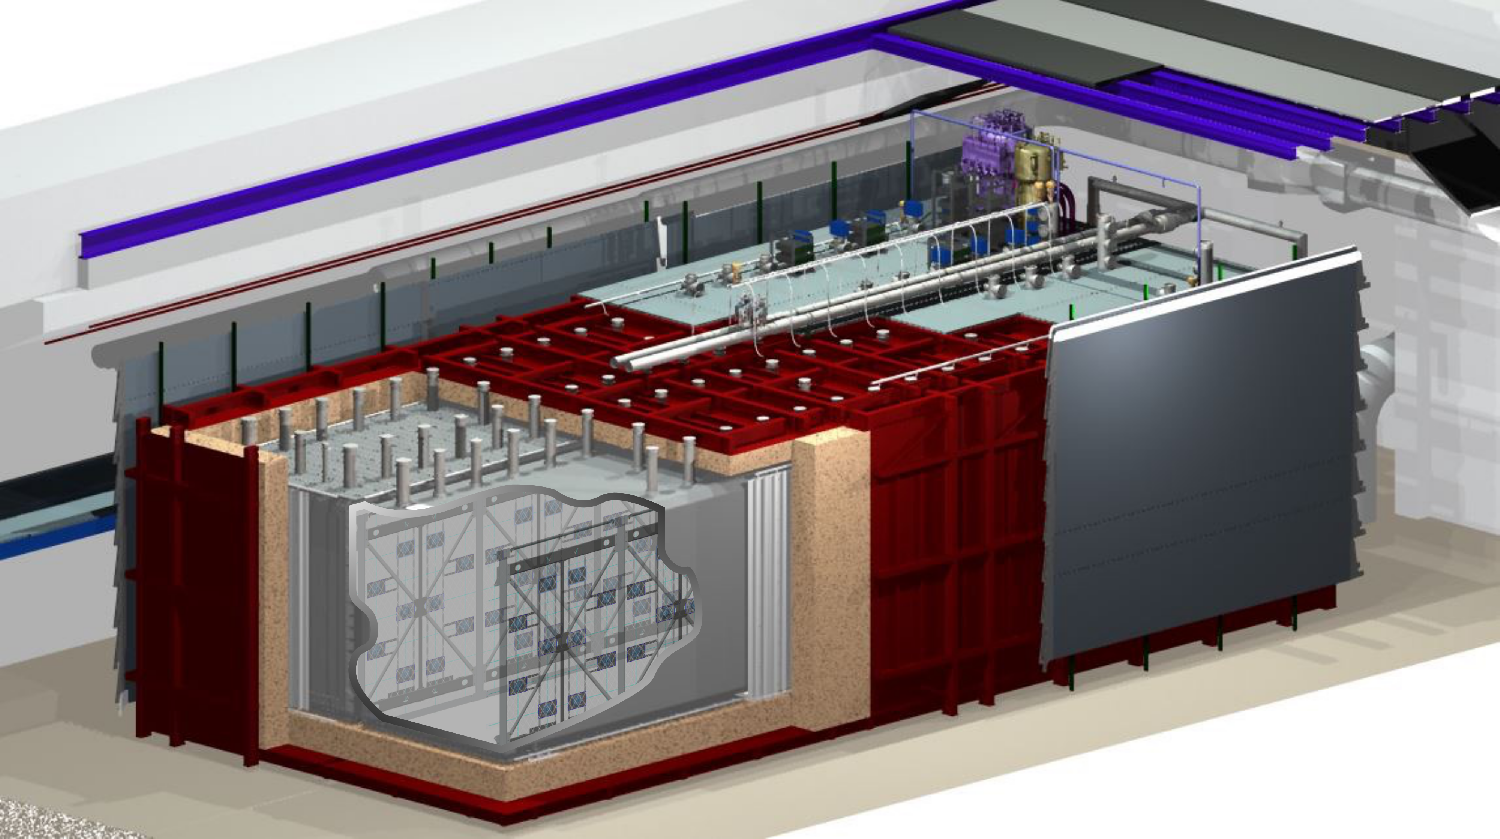
\includegraphics[width=\linewidth]{detector/SBN-FD_composite}};

        \draw[-*, white] (-1,2.5) node [left, white, fill=Gray!15!black] {TPC electronics} -- (0.5,2.25);
        \draw[-*, white] (-9,.5) node [right, white, fill=BrickRed] {Warm vessel} -- (-7.25,-1.5);
        \draw[-*, white] (4,2) node [right, white, fill=Plum!50!black] {Cryogenics} -- (3.25,3.5);
        \draw[-*, white] (7,-0.5) node [below, white, fill=Gray!15!black] {Top-CRT} -- (6.5,4);
        \draw[-*, white] (6,-1.75) node [right, white, fill=Gray!15!black] {Side-CRT} -- (5,-1);
        \draw[-*, white] (6,-3) node [above, white, fill=Gray!15!black] {Bottom-CRT} -- (3.5,-3.75);

        \draw[-*, white] (0,-4.5) node [below, white, fill=Gray!25!black] {East T300 cryostat} -- (-1,-3.5);
        \draw[-*, white] (-4.5,-4.5) node [left, white] {
            \begin{minipage}{4cm}
                \raggedleft
                TPC wireplanes + PMTs
            \end{minipage}} -- (-2.5,-2.5);

        \draw[-Latex, white] (-7,-3.5) -- (-7, -2.5) node[above] {$y$};
        \draw[-Latex, white] (-7,-3.5) -- (-6, -3.2) node[right] {$z$ (beam)};
        \draw[-Latex, white] (-7,-3.5) -- (-7.5, -3.35) node[left] {(drift) $x$};

        \draw[-*, black] (-4.5,5) node [left, black] {\SI{3}{m} concrete overburden} -- (-3,4.5);

        % \draw[step=1.0,white,thin] (-10,-5.5) grid (10,5.5);
        % \foreach \i in {-10,...,10} {
        %     \node [below] at (\i,-5.5) {$\i$};
        % }
        % \foreach \i in {-5,...,5} {
        %     \node [left] at (-10,\i) {$\i$};
        % }

        
    \end{tikzpicture}
    \caption[ICARUS detector illustration]{Illustration of the ICARUS T600 detector at Fermilab. Surrounding the warm vessel is the $4\pi$ coverage CRT. Above the warm vessel, the TPC readout warm electronics are placed, alongside the proximity cryogenics. Inside the warm vessel two identical (east and west) T300 modules are hosted, each containing two TPCs sharing a common cathode at the centre and two anode plane assemblies, one on each side.}
    \label{fig:ICARUS_scheme}
\end{sidewaysfigure}

\subsection{The ICARUS subsystems}

\paragraph{TPC}

\paragraph{Light collection system}

\paragraph{Cosmic ray tagger}


% Firstly proposed by Nobel laureate Carlo Rubbia \cite{Rubbia:1977zz}, the concept of Liquid Argon Time Projection Chambers (LArTPCs for short) was implemented in the Gran Sasso National Laboratories (LNGS) near L'Aquila (Italy) in the ICARUS (Imaging Cosmic And Rare Underground Signals) detector \cite{Bettini:1991fh, Cennini:1994pk, Cennini:1995tt, ICARUS:1995nrd}, which collected data between 2006 and 2011 \cite{Rubbia:2011ft}, alongside the OPERA, LVD and BOREXINO detectors from the CERN Neutrinos to Gran Sasso (CNGS) neutrino beam \cite{Kodama:2004db}. The main detectors for this project were the OPERA and ICARUS experiments, and were therefore called respectively CNGS1 and CNGS2.

% Today, the ICARUS T600 detector is one of the longest running LArTPC in existence. 

% After the results of the CNGS analysis were published the ICARUS detector moved in 2018 from LNGS, to the CERN facility, where it underwent a series of upgrades, both for electronics and in the liquid Argon purification system; serious upgrades were also performed on the exterior of the experiment where a cosmic ray tagger module was added; in 2020 the detector arrived to its current location in the SBN facility at Fermilab, where it has been detecting neutrinos since: mainly $\PGnGm$ and some $\PGne$s, from the Booster Neutrino Beam (BNB, on axis with the $z$ direction of the detector frame of reference) and from the Neutrino Main Injector (NuMI). 

% At the Short Baseline Neutrino (SBN) facility, the ICARUS experiment started its data run taking period in 2022 and has since ran thrice \cite{ICARUS:2023gpo}, with the latest data expected to be ready for the end of 2024 for the official analysis. Its younger brother, the SBND (Short Baseline Near Detector) experiment, finished the cryostat commissioning with some delays in 2023 and is now completing the commissioning of the cosmic ray tagger (CRT) modules, with the analysis on veto efficiency for the top CRT modules ongoing. 

% Joint efforts of the SBND and ICARUS detectors in the SBN collaboration will provide a highly efficient identification of neutrino interactions, strongly mitigating the possible sources of background and reducing the impact of systematics. 

% The combination of two nearly identical detectors allows for the measurement of neutrino oscillations over the distance in between the experiments, comparing the $\nu$s flux at \SI{110}{\meter} (SBND) and at \SI{600}{\meter} (ICARUS). 

% A third and a fourth experiment were also active in the BNB baseline, MiniBooNE (\mboone) and MicroBooNE (\uboone). The former completed its data taking period in 2018, and the latter was active between 2015 and 2021. Those two experiments provided strong ($\sim5\sigma$) evidence of event excess \cite{MiniBooNE:2018esg} in respect to what was expected (see figure \ref{fig:miniboone_results}). The main goal of the SBN collaboration is therefore to test this anomaly using data from BNB neutrinos. 

% In addition to this anomaly, ICARUS will also test the oscillation signal reported by the Neutrino-4 collaboration, hinting towards $\Delta m^2 \simeq \SI{7.26}{\electronvolt\squared}$ and $\sin^22\theta = 0.38$ ($3.5\sigma$ CL), both in $\PGne$ and $\PGnGm$ channels from BNB and NuMI.
% !TEX root=../main.tex

\chapter{Automatic event recontruction in TPC using Pandora}

% !TEX root=../main.tex

\chapter{Validating the automatic Pandora-based reconstruction}
% !TEX root=../main.tex

\chapter{Conclusions}\label{chap:conclusions}

\dictum[Anonymous]{I conclude that when I'm done with my thesis, life will be better}



% \backmatter
\appendix

\chapter{Acronyms}

Throughout the thesis, multiple acronyms or concepts are presented and used; here are the most common with some context

\begin{abbreviations}
    BNB & Booster Neutrino Beam, the main beam feeding the SBN experiment \\
    ICARUS \newline \emph{or SBN-FD} & The name stands for \emph{Imaging Cosmic And Rare Underground Signals}, as it was called in the Gran Sasso era. It is the \SI{760}{\tonne} Far Detector in the SBN experiment \\
    LArTPC & Liquid Argon Time Projection Chamber \\
    SBN & The Short Baseline Neutrino experiment, consisting of the three detectors on the BNB baseline \\
    SBND & Short Baseline neutrino Near Detector \\ 
\end{abbreviations}


% % !TEX root=../main.tex

\chapter{Cheating the track/shower MVA module}

Pandora developers already provide a valid module that cheat the true information for the track/shower classification stage. This fills the PFO metadata with the correct pdg, i.e. assigns pdg $= \pm 13$ \emph{iff} the particle is \PGmpm; 

For the analysis performed in this work the 

\lstinputlisting[style=xmlstyle, language=XML]{7_listings/PandoraSettings_Neutrino_cMva.xml}


\bibliographystyle{5_bsts/utphys}
% \bibliography{4_references/references, 4_references/bibsets, 4_references/Theses}
\bibliography{thesis/4_references/EXPERIMENTAL/experimentalICARUS,thesis/4_references/THEORY/theoryNeutrinos, thesis/4_references/THEORY/theorySterile, thesis/4_references/THEORY/theoryThesis} 

\end{document}
